\documentclass[a4paper]{article}
\usepackage{geometry}
\usepackage{graphicx}
\usepackage{epsfig}
\usepackage{amsmath}
\usepackage{indentfirst}
\usepackage{float}
\usepackage{setspace}
\usepackage{amsfonts}
\usepackage[hidelinks]{hyperref} 
\usepackage{booktabs}
\usepackage{caption}
\usepackage{subfigure}
\usepackage{times}
\usepackage{hyperref}
\usepackage{verbatim}
\usepackage{colortbl}
\usepackage{lscape}
\usepackage[affil-it]{authblk}
\usepackage{footnotebackref}
\usepackage[natbibapa,nodoi]{apacite}
\AtBeginDocument{\urlstyle{APACsame}}
\AtBeginDocument{\renewcommand{\APACrefYearMonthDay}[3]{\BBOP{#1}\BBCP}}


\geometry{left=2cm,right=2cm,top=2cm,bottom=2cm}

\setlength{\parindent}{2em}

\begin{document}
	
	\title{Narrative Conservatism}

	\author{\vspace{1cm}Juan Manuel Garc\'ia Lara}
	
	\author{Beatriz Garc\'ia Osma}
	
	\author{Fengzhi Zhu%
		\thanks{Email: fzhu@emp.uc3m.es}}
	
	\affil{Department of Business Administration, Universidad Carlos III de Madrid, Spain}
	
	\date{\small Dated: \today}
	
	\maketitle
	
\thispagestyle{empty}
\begin{spacing}{2}

\begin{abstract}
	\begin{normalsize}
	\noindent
	Prior literature documents the existence of conditional and unconditional conservatism, which are measured by recognized line items in financial statements. However, little is known about conservatism in narrative disclosure. We investigate whether narrative disclosure is conservative, i.e., whether narratives respond to bad news in a more complete, news-consistent and timely manner than good news. We proxy news by market returns and measure completeness by the number of words, news-consistency by the sign agreement between narrative tone and the nature of news, and timeliness by the reporting time lag between news release date and disclosure reporting date. Using 10-Q and 8-K filings from 1993 to 2020, we find that on average narratives are lengthier, more news-consistent and timelier in response to bad news relative to good news, consistent with narratives being conservative. In addition, we show that firms emphasize bad news more than good news via 10-Q filings, and report more number of 8-K items and filings per day in response to bad news comparing to good news.
	%[auxiliary analysis]% 
	%[Contribution: We contribute to the literature on accounting conservatism by providing evidence of asymmetric narrative disclosure in response to good versus bad news.]% 
	\\

	\noindent
	\textbf{Keywords}: \textit{narrative disclosure; conservatism; asymmetric disclosure; tone; textual analysis}
	\end{normalsize}
\end{abstract}

\clearpage

\setcounter{page}{1}
\section{Introduction}
% motivation
Extant literature documents the existence of recognition conservatism\footnote{In this paper, we use the term ``recognition conservatism" to denote the union of conditional and unconditional conservatism, whose measurements are both derived from recognized line items in financial statements.}. In this paper, we add to this prior work by defining and providing evidence of narrative conservatism. We define narrative conservatism as \textit{narratives responding to bad news in a more complete, news-consistent and timely manner than good news}. This definition builds on the work of \citet*{basuConservatismPrincipleAsymmetric1997}, extending the notion of accounting conservatism to narratives. Narrative conservatism is of interest for at least two reasons. First, narrative disclosure takes up a dominant space in corporate filings\footnote{For example, Apple Inc.'s 2019 Annual Report contains only 3 pages of numerical summary in the financial statements and around 15 pages of other tables and figures, among a total of 64 pages. The rest of the report is devoted to narratives including risk factors, management discussion and analysis (MD\&A), notes to financial statements, among other things. Also, over the past 20 years, the average number of pages in annual reports devoted to footnotes and MD\&A has quadrupled \citep{eyPointNowTime2012}.}. Investors' perception of firm performance and subsequent decision-making process are likely to be shaped by narrative disclosures \citep*{liTextualAnalysisCorporate2010}. Therefore, understanding the properties of narrative disclosure and their economic implications is essential for market participants and regulators. Second, from researchers' point of view, studying narrative conservatism complements our current understanding of accounting conservatism. If recognition is merely one of the presentation formats of financial reporting, then our extant knowledge of recognition conservatism is a partial view of accounting conservatism, which would be comprised of both recognition and narrative conservatism. Yet, we know little about whether narrative disclosure is conservative, or whether and how narrative and recognition conservatism interact with each other.

%[Theory]
Prior literature distinguishes between recognition and disclosure. Recognition is depictions in numbers with captions on the face of the financial statements. In spite of the lack of a conceptual definition, disclosure is commonly viewed as display in the notes and supporting schedules that accompany financial statements \citep*{schipperRequiredDisclosuresFinancial2007}. The two forms of financial reporting are subject to different reporting requirements. The Financial Accounting Standards Board (FASB) explicitly specifies a set of recognition criteria while allowing for more flexibility in disclosure \citep*{fasbStatementFinancialAccounting1984}. This flexibility in disclosure paves a way for one of the two fundamental functions of disclosure---disclosing information that cannot be recognized due to failures to meet one or more of the recognition criteria. The other function of disclosure is to explain recognized numbers in financial statements, that is, to provide supplementary information of line items. 

Extensive research has been conducted on conditional and unconditional conservatism. Conditional conservatism captures the asymmetric response of \textit{earnings} to positive and negative stock returns, and unconditional conservatism manifests as a systematic understatement of \textit{net book value of assets} due to predetermined aspects of the accounting process \citep[e.g.,][]{beaverConditionalUnconditionalConservatism2005}. However, conservatism in narrative disclosure receives little attention. The most related literature investigates whether managers disclose or withhold bad news, using a variety of disclosure proxies except linguistic properties of narratives \citep*{baoManagersDiscloseWithhold2019, kothariManagersWithholdBad2009, skinnerWhyFirmsVoluntarily1994, skinnerEarningsDisclosuresStockholder1997}. Narrative conservatism requires managers to disclose bad news rather than withhold it. Prior studies provide mixed evidence on this debate, but outline several incentives for managers to disclose or withhold bad news. For instance, lower financing costs resulting from reduced information asymmetry, litigation risk due to the failure to disclose bad news in a timely manner and managers' personal incentive to downward manipulate firm performance prior to stock option grant constitute the three major motives for disclosing bad news. On contrary, managers' future career concern and performance-based compensation induce managers to withhold bad news. Given various incentives to disclose and withhold bad news, on average, whether managers tend to disclose or withhold bad news remains an empirical question.

%[research design]
To empirically test whether narrative disclosure is conservative, we adopt the following three measurements for completeness, news-consistency and timeliness respectively. We proxy disclosure completeness by the number of total words in corporate filings. Prior literature documents that managers use lengthier reports to disclose more information, which reduces information asymmetry and lowers cost of capital \citep*{leuzDisclosureCostCapital2009}. We measure news-consistency by the sign agreement between the linguistic tone in corporate filings and the nature of news. That is, positive tone corresponds to good news and negative tone to bad news. The tone of conservative narrative disclosure should be more elastic to bad news than to good news. We evaluate timeliness by the reporting time lag between news and disclosure release dates. The smaller the reporting time lag is, the timelier the narrative disclosure is. Overall, we posit that if narrative disclosure is conservative, it should be lengthier, more news-consistent and timelier in response to bad news than to good news. In terms of news measurement, we follow \citet{basuConservatismPrincipleAsymmetric1997} and apply stock returns to assess the nature of news, assuming market efficiency.

%[data and findings]
We use two types of mandatory filings required by U.S. Securities and Exchange Commission (SEC) for all public companies---10-Q and 8-K filings---as our narrative disclosure corpora. To begin with, we retrieve 10-Q and 8-K filings from the Electronic Data Gathering, Analysis, and Retrieval system (EDGAR) from 1993 to 2020\footnote{Since the SEC adopted the rule of electronical submission for corporate filings in 1993, data coverage in the first year of EDGAR implementation is low \citep*{gaoInformingMarketEffect2020}. We repeat our main analyses using data from 1994 onward, and our main results sustain.}. Next, we apply the financial sentiment word list developed by \citet*{loughranWhenLiabilityNot2011} (LM hereafter) to count number of positive, negative, uncertainty, litigious and modal words in each corporate filing extracted from EDGAR. Finally, we construct tone as the number of net positive words per thousand total words and reporting time lag as number of days elapsed between news release date and document reporting date. Our final 10-Q (8-K) sample consists of 91,606 (244,401) firm-quarter (firm-day) observations from 5,250 (8,876) unique firms. Empirical results show that 10-Q (8-K) filings are lengthier, more news-consistent, and less (more) timely in response to bad news relative to good news, generally consistent with narrative disclosures being conservative\footnote{All empirical results are consistent with narratives being conservative except that 10-Q filings responding less timely to bad news than good news, which contradicts with narrative conservatism. However, because 10-Q is not as timely as 8-K, and because 10-Q report not only contains narrative disclosures but also financial statements, it does not strictly proxy for narrative timeliness (\hyperref[sec3.1]{Section 3.1}). Therefore, we interpret 10-Q results only as a supplementary evidence when it comes to narrative timeliness. The main conclusions regarding narrative timeliness are drawn based on 8-K results.}. 

%[auxiliary analysis]

%[contribution]
This paper contributes to the accounting literature in four aspects. First, we fill the missing piece in conservatism literature by documenting the existence of narrative conservatism. Second, we provide novel evidence to the debate regarding whether managers withhold bad news \citep{baoManagersDiscloseWithhold2019, kothariManagersWithholdBad2009, skinnerWhyFirmsVoluntarily1994, skinnerEarningsDisclosuresStockholder1997}. We apply linguistic properties of SEC filings as proxy for disclosure, and our results support the idea that firms voluntarily disclose bad news on average. [Third, we add to the literature on distinction and interaction between recognition and disclosure \citep*{schipperRequiredDisclosuresFinancial2007, barthMarketEffectsRecognition2003, aboodyRecognitionDisclosureOil1996}. Fourth, we relate to the broader literature on the informativeness of SEC filings \citep*{lermanNewForm8K2010, alfordExtensionsViolationsStatutory1994, liAnnualReportReadability2008, liInformationContentForwardLooking2010}, suggesting that 10-Q and 8-K filings are incrementally informative in response to bad news relative to good news.]\footnote{ The third and fourth contributions are yet to be confirmed by auxiliary analyses.}

The rest of the study structures as follows. Section 2 reviews prior literature on recognition, disclosure, conditional and unconditional conservatism, and develops the main hypotheses. Section 3 outlines the empirical design and data selection process. Section 4 presents the main results of 10-Q and 8-K samples. Section 5 performs auxiliary analyses and Section 6 concludes.

\section{Theoretical Framework}
\subsection{Recognition and Disclosure}
A longtanding literature studies the distinctions between \textit{recognition} and \textit{disclosure} and their respective or combined effectiveness in financial reporting \citep*{schipperRequiredDisclosuresFinancial2007, barthMarketEffectsRecognition2003, aboodyRecognitionDisclosureOil1996}. \citet[p. 301]{schipperRequiredDisclosuresFinancial2007} defines recognition as ``depictions in numbers with captions on the face of the financial statements", and disclosure as ``display in the notes and supporting schedules that accompany financial statements"\footnote{Statement of Financial Accounting Concepts No. 5---\textit{Recognition and Measurement in Financial Statements of Business Enterprises} formally defines \textit{recognition} as ``the process of formally recording or incorporating an item into the financial statements of an entity as an asset, liability, revenue, expense, or the like. Recognition includes depiction of an item in both words and numbers, with the amount included in the totals of the financial statements" \citep*[par. 6]{fasbStatementFinancialAccounting1984}, but does not define \textit{disclosure}. Due to the absence of a conceptual definition of disclosure, prior literature on disclosure commonly interpret disclosure as any display that is not in numbers. However, this interpretation may partially overlap with the FASB definition of recognition, which states that recognition also includes words. As \citet[p. 302]{schipperRequiredDisclosuresFinancial2007} notes: ``...both in analytical modeling and in developing financial reporting concepts, it is difficult to distinguish between recognized and disclosed information".}. In this study, we adopt the same notion of recognition as in \cite{schipperRequiredDisclosuresFinancial2007}, and we use the terms \textit{narratives, narrative disclosure} or \textit{disclosure} interchangeably to denote all textual disclosures presented in SEC filings, including notes to financial statements, supplementary information and other means of financial reporting such as MD\&A section. Examples of recognition are revenue, expense, asset and liability expressed in currency units on the face of financial statements, which are also known as line items in financial statements. 

Disclosure and recognition are subject to different reporting requirements. For an economic item to be recognized in financial statements, a set of recognition criteria needs to be satisfied. First, the item must meet the definition of an element of financial statements (definition criterion). Second, the item must have a relevant attribute measurable with sufficient reliability (measurability criterion). Third, the information about the item must be capable of making a difference in user decisions (relevance criterion). Fourth, the information must be representationally faithful, verifiable, and neutral (reliability criterion) \citep{fasbStatementFinancialAccounting1984}. However, disclosure is more flexible because it is can be deployed to disclose information that fail to meet certain recognition criteria. 

Narrative disclosure plays an essential role in financial reporting, as \citet*[par. 7]{fasbStatementFinancialAccounting1984} states:

\textit{Although financial statements have essentially the same objectives as financial reporting, some useful information is better provided by financial statements and some is better provided, or can only be provided, by notes to financial statements or by supplementary information or other means of financial reporting.}

Concretely, narrative disclosure has two fundamental functions. First, narrative disclosure may convey information about corporate events that cannot be recognized, due to the inability to meet one or more of the four recognition criteria. For instance, firms may not recognize losses that could result from a potential lawsuit in the future since it is extremely difficult to obtain a reliable estimate that can be verified subsequently, considering the reputation damage. However, firms may discuss the likelihood and impact magnitude of entering into a lawsuit in risk factor or MD\&A section of 10-Q/K filings. Treatment for intangible assets serves as another example where narrative disclosure is able to convey information that is not allowed to be recognized in financial statements. Internally developed intangible assets cannot be capitalized in the balance sheet, so they cannot be impaired when bad news arrives. However, firms may discuss the impact of news associated with these intangible assets in SEC filings. In sum, firms may use narrative disclosure to inform investors about the immeasurable, and thus irrecognizable impact of various corporate events and fulfill their obligation of providing relevant financial information to investors. Second, narrative disclosure may explain the line items in financial statements. \citet*[footnote 4]{fasbStatementFinancialAccounting1984} gives several examples on the explanatory role of notes to financial statements:

\textit{For example, notes provide essential descriptive information for long-term obligations, including when amounts are due, what interest they bear, and whether important restrictions are imposed by related covenants. For inventory, the notes provide information on the measurement method used---FIFO cost, LIFO cost, current market value, etc. For an estimated litigation liability, an extended discussion of the circumstances, counsel's opinions, and the basis for management's judgment may all be provided in the notes. For sales, useful information about revenue recognition policies may appear only in the notes (FASB Statement No. 47, Disclosure of Long-Term Obligations; ARB No. 43, Chapter 4, ``Inventory Pricing", statement 8; FASB Statement No. 5, Accounting for Contingencies, par. 10; and APB Statement 4, par. 199)}.

\subsection{Recognition and Narrative Conservatism: Definition}

Prior literature documents conservatism in two forms: conditional and unconditional conservatism. Conditional conservatism, or earnings conservatism, is defined as ``accountants' tendency to require a higher degree of verification to recognize good news as gains than to recognize bad news as losses" \citep*[p. 7]{basuConservatismPrincipleAsymmetric1997}, and is measured by the asymmetric response of earnings to positive and negative stock returns. Examples of conditional conservatism include allowing for \textit{impairment}, i.e., writing down by the amount of loss incurred, but not \textit{revaluation}, i.e., writing up by the difference between market price and carrying amount, for long-lived tangible and intangible assets under U.S. General Accepted Accounting Principle (GAAP), and lower of cost or market accounting (LCM) for inventory under U.S. GAAP or lower of cost or net realizable value accounting (LCNRV) under International Financial Reporting Standards (IFRS). Unconditional conservatism, or balance sheet conservatism, is defined as ``accountants' preference for accounting methods that lead to lower reported values for shareholders' equity" \citep*[p. 8]{basuConservatismPrincipleAsymmetric1997}. Examples of unconditional conservatism include immediate expensing, rather than capitalizing, research and development (R\&D hereafter) costs, and the use of accelerated depreciation method for property, plant and equipment \citep*{beaverConditionalUnconditionalConservatism2005}. The measurements of both types of conservatism---earnings and shareholders' equity, are recognized line items in financial statements. Thus, we label the union of the two forms of conservatism as \textit{recognition conservatism}. 

Comparing to the extensive research on recognition conservatism, little is known about conservatism in narratives. We define narrative conservatism as \textit{narratives responding to bad news in a more complete, news-consistent and timely manner than good news}. Narrative conservatism implies that firms should disclose bad news rather than withhold it. While prior literature shows mixed evidence on firms' tendency to disclose or withhold bad news, several explanations are proposed as to why managers disclose or withhold bad news. On the one hand, managers may choose to disclose bad news for three motives. First, managers may disclose more complete information, including bad news, in order to reduce financing costs. Extant theoretical work establishes that complete disclosure reduces information asymmetry and lowers cost of capital \citep[e.g.,][]{diamondDisclosureLiquidityCost1991, baimanRelationCapitalMarkets1996}. \citet*{leuzEconomicConsequencesIncreased2000} show that information asymmetry is reduced after German firms switching from the German to an international reporting regime, thus increasing their level of disclosure. \cite{leuzDisclosureCostCapital2009} find that firms respond to the adverse shock created by Enron scandal by increasing length of disclosures in 10-K fillings, which in turn mitigates the impact of transparency crisis. Second, litigation pressure induces managers to disclose bad news more promptly than good news \citep*{skinnerWhyFirmsVoluntarily1994, skinnerEarningsDisclosuresStockholder1997, kasznikWarnNotWarn1995}. Financial information users have greater incentive to sue the manager when the latter fails to disclose bad news than good news. This asymmetric litigation pressure potentially stems from users' asymmetric preference for unexpected gain and losses. Third, the personal career and compensation incentives also play a role in managers' decisions to disclose bad news. \citet{skinnerWhyFirmsVoluntarily1994} argues that managers may face reputational costs if they fail to disclose bad news. \citet*{yermackGoodTimingCEO1997} and \citet*{aboodyCEOStockOption2000} document that managers release bad news immediately prior to stock option grant dates in order to lower the option strike price. On the other hand, managers may withhold bad news for two reasons. First, managers may avoid disclosing bad news for career concerns, in expectation to bury bad news with subsequent corporate events. Significant bad news affects managerial career negatively by deterring promotion, limiting employment opportunity in the outside job market and potentially leading to termination. Second, performance-based managerial compensation also demotivates managers to disclose bad news. Bad news disclosure may lead to bonus shrink and stock price decline, reducing managers' personal wealth especially when they are compensated with shares or options \citep{kothariManagersWithholdBad2009}. In sum, while managers have a natural tendency to disclose good news, they face different incentives when it comes to the decision of disclosing or withholding bad news. Given various managerial incentives presented, whether narratives on average disclose bad news in a more complete, news-consistent and timely manner than good news or not remains an empirical question.

To investigate this question, we construct three measurements for disclosure completeness, news-consistency and timeliness respectively. We measure disclosure completeness by the total number of words of SEC filings. Because the Conceptual Framework requires complete disclosures to include ``...all information necessary for a user to understand the phenomenon being depicted, including all necessary descriptions and explanations" \citep*[QC12]{fasbConceptualFrameworkFinancial2018}, more complete disclosures should manifest as lengthier documents, which allow managers to elaborate detailed descriptions and explanations of firm performance \citep{leuzDisclosureCostCapital2009}\footnote{We use number of words instead of number of pages, which is used in \citet{leuzDisclosureCostCapital2009}, as the proxy for disclosure completeness for two reasons. First, for pure texts, these two measures are almost equivalent, or at least are monotonic transformations of each other, given a roughly constant number of words per page. Second, for financial report with graphs and tables, the number of words is a more precise measure for narrative disclosure, because it counts the length of narratives only. However, the number of pages may be enlarged by graphs, tables, and even space lines embedded in the tables, which are not focus of this study.}. However, a strand of literature documents that narrative disclosure is less informative when it is less readable \citep*{liAnnualReportReadability2008, loEarningsManagementAnnual2017, loughranMeasuringReadabilityFinancial2014}, and because lengthier document is often less readable, it may appear counter-intuitive to proxy completeness with document length. We provide two explanations for this measurement. First, several studies point out that instead of managers' intentional obfuscation, lower readability may result from the fact that bad news is inherently more complex and therefore needs more explanations \citep*{bloomfieldDiscussionAnnualReport2008}, and that there is incremental information content embedded in complex narratives \citep*{busheeLinguisticComplexityFirm2018}. Therefore, lower readability does not necessarily imply lower narrative disclosure quality. Second, although somewhat correlated, document length and readability are essentially two different constructs. In a binary classification context, texts can be long or short, readable or irreadable independently. Specifically in measuring information completeness, document length is an appropriate construct because ``including all necessary descriptions and explanations" \citep*[QC12]{fasbConceptualFrameworkFinancial2018} in narrative disclosure inevitably increases document length. Thus, if narrative disclosure is conservative, we expect it to be lengthier in response to bad news. We formulate our first hypothesis as follows:

\begin{center}
	\begin{tabular}{l}
		\textbf{H1:} Narrative disclosure is lengthier in response to bad news than good news.
	\end{tabular}
\end{center}

We measure the sentiment spectrum in narrative disclosure with linguistic tone. By consistency we mean the sign agreement between disclosure tone and nature of news, i.e., the correspondence of positive tone to good news and negative tone to bad news. If the tone of narrative disclosure is more news-consistent in response to bad news than to good news, it implies higher tone elasticity for bad news than for good news. That is, the disclosure tone is more negative in response to bad news than it is positive in response to good news, given the same magnitude of news impact. Narrative conservatism creates a downward bias in narrative disclosure conditional on the nature of news: either bad news is emphasized or good news is attenuated, or both. Thus, we formulate our second hypothesis as follows:

\begin{center}
	\begin{tabular}{l}
		\textbf{H2}: Narrative disclosure tone is more news-consistent in response to bad news than good news.
	\end{tabular}
\end{center}

We measure timeliness by the reporting time lag, defined as the number of days elapsed between the news release date and subsequent reporting date of the narrative disclosure. In line with the interpretation of timeliness in the Conceptual Framework that ``Timeliness means having information available to decision makers in time to be capable of influencing their decisions" \citep*[QC29]{fasbConceptualFrameworkFinancial2018}, the shorter is the reporting time lag, the timelier is the narrative disclosure. If narrative disclosure is conservative, we expect it to be timelier in response to bad news. Thus, we formulate our third hypothesis as follows:

\begin{center}
	\begin{tabular}{l}
		\textbf{H3}: Narrative disclosure is timelier in response to bad news than good news.
	\end{tabular}
\end{center}

\subsection{Recognition and Narrative Conservatism: Usefulness}
%[conservatism role: stewardship or neutrality]
The controversy regarding whether conservatism is a desirable property that enhances the usefulness of financial reporting persists. Traditionally, the usefulness of accounting information can be assessed in terms of how well it serves each of the two objectives of accounting---valuation and stewardship. The valuation objective is to ``provide financial information about the reporting entity that is useful to existing and potential investors, lenders, and other creditors in making decisions about providing resources to the entity \citep[OB2]{fasbConceptualFrameworkFinancial2018b}". For financial information to be useful for valuation objective, it must be relevant and faithfully represent what it purports to represent. Faithful representation further requires neutrality, which means that a depiction must be ``not slanted, weighted, emphasized, deemphasized, or otherwise manipulated to increase the probability that financial information will be received favorably or unfavorably by users". The stewardship objective is to assess ``how efficiently and effectively the entity's management and governing board have discharged their responsibilities to use the entity's economic resources \cite[OB4]{fasbConceptualFrameworkFinancial2018b}". Although not separately stated in the Conceptual Framework as one primary purpose of financial reporting, the stewardship role of accounting dates back several millennia and has been one of the main reasons for the existence of accounting \citep{lennardStewardshipObjectivesFinancial2007, murphyDiscoursesSurroundingEvolution2013, pelgerPracticesStandardsettingAnalysis2016}. On the one hand, conservatism contradicts the valuation role of accounting by introducing downward bias in financial reporting and thus weakening its ability to faithfully represent firm performance. For example, unconditional conservatism encourages firms to anticipate and recognize losses before their realization, resulting in a systematic downward bias in asset valuation \citep*[e.g.,][]{wattsPositiveAccountingTheory1986}. Conditional conservatism requires higher verification for good news to be recognized than bad news, leading to asymmetric timeliness in gain and loss recognition in earnings \citep*[e.g.,][]{basuConservatismPrincipleAsymmetric1997}. On the other hand, conservatism enhances the stewardship role of accounting by providing verifiable financial information and thus improving contract efficiency. For example, in debt contracting the unconditional conservatism gives lenders a verifiable lower bound of current value of net assets, which can be used as input for loan decisions. Also, in compensation contracting conditional conservatism limits managers' ability to overstate earnings in order to maximize personal wealth at the expense of other claimholders \citep*[e.g.,][]{wattsConservatismAccountingPart2003}.

% Financial Accounting Standards Advisory Council (FASAC) had a fierce discussion on the clash between neutrality and conservatism and finally decided to include the former and exclude the latter from Conceptual Framework \citep*{fasacFASACMeetingHandouts2005}.

Aligned with the prior literature on the usefulness of conservatism, we argue that more complete, news-consistent and timely disclosure of bad news relative to good news enhances contract efficiency [specific hypotheses to be developed]. However, we do not make claims about the valuation role of narrative conservatism.

\section{Research Design}
\subsection{Narrative Disclosure Corpora and News Proxy} \label{sec3.1}
% Why 10-Q and 8-K?
In this paper, we study narrative disclosure using 10-Q and 8-K filings from EDGAR database as our corpora. The form 10-Q is a comprehensive report that depicts quarterly firm performance, and it must be filed by all public companies to SEC within 40 (for accelerated filers) or 45 days (for all other registrants) after fiscal quarter-end, according to Section 13 or 15(d) of the Securities Exchange Act of 1934. The form 8-K is a report that all public firms must file to the SEC in order to notify investors about material events or changes in the company. 8-K filings must be filed upon the occurrence of any one or more events pertaining to a wide set of pre-specified corporate events, where each type of event is classified as an \textit{8-K item}\footnote{See the list of 8-K items in \hyperref[appd]{Appendix D}.}. Firms can issue narrative disclosures via multiple channels, such as social media and press, conference calls and annual reports etc. We focus on 10-Q and 8-K filings in this study for three motives. First, 10-Q and 8-K are both firm-issued filings that are mandatory for all public companies. Their content is under SEC scrutiny and biased reporting increases litigation risk \citep*{rogersDisclosureToneShareholder2011, cazierWhenAreFirms2020}. Therefore, 10-Q and 8-K filings provide higher credibility comparing to firm-issued disclosures via social media and press. Second, 10-Q and 8-K filings are highly scripted and have higher reporting threshold comparing to conference calls, meaning that corporate events need to have a moderate impact on firm operations in order to be discussed in 10-Q and 8-K filings \citep*{hassanFirmLevelPoliticalRisk2019}. Thus, we filter out less relevant events and concentrate on the ones with moderate impact by using 10-Q and 8-K reports. Third, 10-Q and 8-K filings are timelier than 10-K filings, i.e., annual reports. Using 10-K filings, managers can only bundle information acquired during the whole fiscal year and make summarized responses to all events in one single report at year-end. Given that one of our goals is to examine the timeliness of narrative disclosures, 10-K filings cannot provide sufficient time variation in good and bad news responses, and thus they are not appropriate text source for the purpose of this study.

% Advantage and disadvantage of 10-Q and 8-K?
There is heterogeneity between 10-Q and 8-K filings as well. First, 10-Q filings provide more variation and diversity in content than 8-K filings. 10-Q contains sections such as notes to financial statements and MD\&A, where managers can discuss the economic implications of significant corporate events and issue forward-looking statements, while 8-K filings only offer descriptive texts of events in standardized format. Moreover, 8-K filings are shorter, i.e. contain fewer words than 10-Q filings on average. These features imply that 10-Q filings are more flexible in content, in the sense that managers have more discretion on what and how to disclose in 10-Q filings, which provides us with more variation in linguistic tone than 8-K filings. Thus, our analyses regarding linguistic tone are mainly conducted on 10-Q sample and our conclusion regarding linguistic tone is mainly drawn based on results from 10-Q sample. 

Second, 10-Q filings are not as timely as 8-K filings. 10-Q filings shall be filed once every quarter, so regardless of managerial reporting incentive, 10-Q filings cannot be as timely as 8-K filings in responding to unexpected corporate events, especially for those events that happen during early days in a fiscal quarter. This is testified by the following excerpt extracted from SEC's announcement of a reform in 8-K item classification regime, which became effective on August 23rd of 2004: 

\textit{Under the previous Form 8-K regime, companies were required to report very few significant corporate events. The limited number of Form 8-K disclosure items permitted a public company to delay disclosure of many significant events until the due date for its next periodic report. During such a delay, the market was unable to assimilate such undisclosed information into the value of a company's securities. The revisions that we adopt today will benefit markets by increasing the number of unquestionably or presumptively material events that must be disclosed currently. They will also provide investors with better and more timely disclosure of important corporate events.}

\begin{flushright}
	\citep[Final Rule: Additional Form 8-K Disclosure Requirements and Acceleration of Filing Date,][]{secFinalRuleAdditional2004}
\end{flushright}

Furthermore, besides narrative disclosure, 10-Q filings also contain quarterly financial statements, so the reporting time lag of 10-Q does not strictly measure the timeliness of narrative disclosure solely, but the timeliness of recognition and disclosure in aggregation. Considering these features, our analyses regarding timeliness are mainly conducted on 8-K sample and our conclusion regarding timeliness is mainly drawn based on results from 8-K sample.

Following \citet{basuConservatismPrincipleAsymmetric1997}, we measure good and bad news with stock returns. This proxy is valid under the assumption of market efficiency. In efficient market, stock returns incorporate public and private information in a timely manner and therefore are indicative of good and bad news of firms. %[cite and development needed]
Then firms respond to news by offering explanations of the events that caused changes in stock returns via 10-Q or 8-K filings. To the extent that we use stock returns measured at date immediately before 10-Q and 8-K report filing date, reverse causality is unlikely to confound our results. That is, the stock returns are not reacting to issuance of corporate filings, but to other events that happen before report filing date.

\subsection{Model Specification}
\subsubsection{Form 10-Q}
10-Q filings are quarterly reports that are filed to SEC within 40 or 45 days after fiscal quarter-end. Given their stable periodicity, we design the following model to explore how 10-Q filings behave when firms face good versus bad news. 
\begin{equation} \label{eq1}
TEX_{i,t}=\beta_0+\beta_1QRET_{i,t}+\beta_2NEG_{i,t}+\beta_3QRET_{i,t}\times NEG_{i,t}+\beta_nCONTROLS_{i,t}+\epsilon_{i,t}
\end{equation}

In Equation (1), QRET denotes the quarterly market-adjusted stock returns. NEG is an indicator for bad news, which is set to 1 if QRET is negative and 0 otherwise. CONTROLS represents a vector of control variables, which includes firm size (SIZE), market-to-book ratio (MTB) and leverage ratio (LEV) (see \hyperref[appc]{Appendix C} for detailed variable definition). We control for these three firm characteristics in order to alleviate the omitted variable bias, as these three factors can affect stock returns and firm narrative disclosure simultaneously \citep*{liInformationContentForwardLooking2010, huangToneManagement2014}. %[specific explanation on each of the controls and cite needed]
Notice that the right-hand side of Equation (1) resembles the conditional conservatism model in \citet{basuConservatismPrincipleAsymmetric1997}. Our model differs from the Basu model in replacing earnings with three textual variables in order to examine the responses of narrative disclosures to positive versus negative market returns. Specifically, TEX represents a vector of textual properties that consists of number of words (NW), tone (TONE) and reporting time lag (TLAG). NW is calculated as the natural logarithm of one plus the count of total words. TONE is defined as number of net positive words per thousand total words, and is calculated as total number of positive words minus the sum of total number of negative words and total number of negations, and multiply the previous result by one thousand for ease of interpretation. We follow \citet{loughranWhenLiabilityNot2011} and count negations as cases where negation words\footnote{Negation words include: no, not, none, neither, never, nobody \citep*{tottieNegationEnglishSpeech1991}.} occur within four or fewer words from a positive word. By taking negations of positive words into consideration in calculating tone, we control for the fact that it is common for firms to frame bad news using negated positive words (“did not profit”). We do not control for negations of negative words because firms rarely communicate good news with negated negative words (“did not fail”). TLAG is defined as number of days elapsed between the news release date and document filing date in EDGAR. One concern of the TLAG measurement for reporting timeliness is that the length of reporting time lag may not be fully controlled by firms, and thus cannot accurately capture the discretionary reporting timeliness of firms, because prior auditing literature suggests that a set of auditor characteristics contributes to unexpected audit report lag \citep*{knechelAdditionalEvidenceAudit2001, bamberAuditStructureOther1993}, which consequently leads to filing delay in audited financial reports. However, because audit for quarterly filings is not mandated by law, and due to the expensive auditing cost, most 10-Q filings are not audited.

The coefficient of interest in Equation (1) is $\beta_3$, which is interpreted as the difference in responsiveness of textual properties to good versus bad news. If 10-Q narrative disclosure is conservative, we expect it to be lengthier, more news-consistent and timelier when firms receive bad news. In the case of NW being the dependent variable, $\beta_3^{NW}$ should be negative under H1, because QRET is always negative when NEG equals 1, and therefore the product of the interactive term $\beta_3^{NW}QRET_{i,t}\times NEG_{i,t}$ is positive, which translate into increased document length in terms of number of words. Following the same logic, $\beta_3^{TLAG}$ of TLAG regression should be positive under H3, which translates into shorter reporting time lag. The interpretation of $\beta_3^{TONE}$ is different from those of the previous two estimations, in the sense that $\beta_3^{TONE}$ represents the incremental consistency between news and tone. We define consistency as the correspondence of positive tone to good news and negative tone to bad news. Under this definition, a positive incremental consistency, reflected as positive $\beta_3^{TONE}$, means that on average, the disclosure tone is more negative in response to bad news than it is positive in response to good news, given the same magnitude of news impact.

Additionally, we construct an abnormal tone measure (ABTONE) following the expected tone model in \citet{huangToneManagement2014}. ABTONE is calculated as the residual of the following model\footnote{Our expected tone model differs from \citet{huangToneManagement2014} in replacing book-to-market ratio with market-to-book ratio.}:
\begin{equation} \label{eq2}
\begin{split}
TONE_{i,t}=\beta_0&+\beta_1EARN_{i,t}+\beta_2RET_{i,t}+\beta_3SIZE_{i,t}+\beta_4MTB_{i,t}+\beta_5STD\_EARN_{i,t}\\
&+\beta_6STD\_RET_{i,t}+\beta_7AGE_{i,t}+\beta_8BUSSEG_{i,t}+\beta_9GEOSEG_{i,t}+\beta_{10}LOSS_{i,t}\\
&+\beta_{11}\Delta EARN_{i,t}+\beta_{12}AFE_{i,t}+\beta_{13}AF_{i,t}+\epsilon_{i,t}
\end{split}
\end{equation}
Where TONE is the number of net positive words per thousand total words. Other financial variables are defined in \hyperref[appc]{Appendix C}. As residuals of Equation (2), ABTONE captures the portion in tone that is orthogonal to firm fundamentals such as business complexity, growth opportunities and risk, and represents the portion subject to managerial discretion. Our regression result of the expected tone model is consistent with \citet{huangToneManagement2014}\footnote{See results comparison for expected tone model in \hyperref[oat1]{Table 1 of Online Appendix}.}.

\subsubsection{Form 8-K}
%%%% 8-K filing data structure
Due to the irregularity of 8-K triggering events, 8-K filings in EDGAR database have a unique data structure: though most companies only report one 8-K filing in one day and each 8-K filing usually contains only one or two 8-K items, some firms report more than one 8-K filings per day and each 8-K filing may contain more than two items. So we construct 8-K sample in three steps. First, as we want to analyze the responsiveness of 8-K filings to good and bad news, and our news proxy---daily stock return is at firm-day level, we aggregate the raw 8-K data at individual event level into 8-K data at firm-day level by summing up all raw count variables over each firm-day. For instance, the count variable $nw_{i,t}$ in 8-K dataset stands for number of total words in all 8-K filings reported in day \textit{t} for firm \textit{i}, instead of number of total words of one specific 8-K filing. In order to keep track of the unique data structure of 8-K filings, we further construct two new variables---N8K and NITEM, which are defined as number of 8-K filings reported in one day and number of 8-K items reported in one day, respectively. We label a firm-day as “8-K day” if there is at least one 8-K filing reported in that day.

%%%% 8-K news proxy
Next, we build our proxy for news under 8-K context. We obtain the daily market-adjusted stock returns (DRET) based on raw data from CRSP and calculate the change in daily returns ($\Delta$DRET). Then, we define a firm-day as a “bad (good) news day” if the negative (positive) change in daily market-adjusted stock return ($\Delta$DRET) is three times larger than the firm's average decrease (increase) in daily return over the calendar year. BN is an indicator for bad news day, which is set to 1 if this firm-day is a bad news day, and 0 if this firm-day is a good news day\footnote{We code BN to missing if the firm-day does not have any news. Therefore, in our final 8-K sample for regression analysis, all observations are either good or bad news firm-days.}. Notice that we define good and bad news differently under 8-K and 10-Q context. This is because that daily returns are more volatile than quarterly returns and the sign of daily returns can change constantly merely due to trading noises. Therefore, we only focus on firm-days with sizable changes in daily returns (three times than annual average), which is more likely to result from significant corporate events and is more likely to reflect fundamental information about the firm.

%%%% 8-K event matching process
At last, we conduct a matching process as illustrated in \hyperref[fig1]{Figure 1}. The idea of matching is to pair the news releases to firms' responses in form of 8-K filings to the precedent news. Specifically, we match every news day to its first subsequent 8-K day, ignoring the successive 8-K days (if any) between two news days (Match-1), or in some cases the 8-K day coincides with news day (Match-2). The underlying assumption behind this matching process is that the first 8-K issued after a news release is indeed responding to that news. We acknowledge the limitation of this assumption: time sequence does not necessarily imply association---that is, the fact that some 8-K filings are reported immediately after certain news does not guarantee that the 8-K filings are meant to address that news\footnote{We will do validation check in the development of the paper.}.
After matching, we calculate TLAG of 8-K sample as the number of days elapsed between the news release date and document filing date\footnote{All filings in EDGAR have two dates: filing date and reporting period date. Filing date is the date when the document is filed to EDGAR, and reporting period date is the end date of reporting period of the filing. We match by 8-K \textit{reporting period date} because we want to make sure that the 8-K filings reported at a specific date are indeed responses to the news released just before. However, we calculate TLAG using 8-K \textit{filing date} because we are interested in whether 8-K filings respond to good and bad news with different timeliness, allowing for managerial discretion in reporting speed.}. 

Once the 8-K sample is constructed, we design the following model to explore how 8-K filings behave when firms have good versus bad news.
\begin{equation} \label{eq3}
TEX_{i,t}=\beta_0+\beta_1\Delta DRET_{i,t-tlag}+\beta_2BN_{i,t-tlag}+\beta_3\Delta DRET_{i,t-tlag}\times BN_{i,t-tlag}+\beta_nCONTROLS_{i,t}+\epsilon_{i,t}
\end{equation}
Where $\Delta$DRET and BN are changes in daily returns and bad news indicator \textit{at news release date}. We deploy $\Delta$DRET rather than DRET in this model because under 8-K context, the bad news indicator BN is defined based on $\Delta$DRET, as opposed to DRET. In Equation (3), CONTROLS denotes a vector of control variables \textit{at 8-K filing date}\footnote{Because our measures of firm fundamentals are calculated based on Compustat quarterly data, the variation in firm fundamental measures is very small (if any) either we control for them at news release date (t-tlag) or at 8-K filing date (t), as the average reporting time lag of 8-K is only 23 days.}, which includes firm size (SIZE), market-to-book ratio (MTB) and leverage ratio (LEV). We control for these three fundamental characteristics that may affect firms reporting policy in order to address the omitted variable bias. TEX represents a vector of textual properties that consists of number of words (NW), tone (TONE) and reporting time lag (TLAG), which share the same definition as in 10-Q context. The coefficient of interest in Equation 3 is still $\beta_3$, and its interpretation is the same as that in the context of 10-Q. If 8-K narrative disclosure is conservative, we expect it to be lengthier, more news-consistent and timelier when firms respond to bad news, which manifests as negative $\beta_3^{NW}$, positive  $\beta_3^{TONE}$ and positive $\beta_3^{TLAG}$.

\subsection{Data}
We obtain historical financial and segment data from Compustat, stock returns from the Center for Research in Security Prices (CRSP) and analyst earnings forecasts data from I/B/E/S. We retrieve 10-Q and 8-K data from EDGAR through a self-developed Python program (see \hyperref[appa]{Appendix A} for detailed description of EDGAR data collection process). \hyperref[T1]{Table 1} illustrates the sample selection process of 10-Q and 8-K filings. First, we successfully parsed and retrieved 575,579 (1,489,626) unique 10-Q (8-K) filings out of 594,017 (1,628,467) existing filings in EDGAR from 1993-Q1 to 2020-Q1. Next, we merge 10-Q and 8-K dataset with other datasets of firm characteristics and market performance. Finally, we screen the merged 10-Q and 8-K dataset according to the following criteria. We eliminate observations with missing value in key accounting and financial variables or with beginning-of-quarter stock prices below \$1. In 10-Q sample, we further delete observations with missing values in analyst coverage variables. We exclude financial (SIC code between 6000 and 6999) and utility (SIC code between 4900 and 4999) firms because the accounting policy for the former is different from that of other industries, and they are both highly regulated industries which are incomparable to other industries in general. Observations with non-positive total assets or book value of equity, or with negative or above 99\% percentile reporting time lag (TLAG)\footnote{Before truncation, the average reporting time lag for 10-Q is 40 days, but the maximum lag is 4,069 days, which is filed by CPI Corp in 2007-06-21 to report a quarterly result as of 1996-04-27 (see \url{https://www.sec.gov/Archives/edgar/containers/fix041/25354/0001140361-07-012753.txt}). We read some of the 10-Q filings with such extremely long reporting lag but do not find an explanation for the unusual delay. In theory 10-Q filings should be filed within 40 or 45 days after fiscal quarter-end, so it remains a puzzle as to why in practice there exists a few accepted filings with such a big delay in EDGAR database. For the purpose of this study we eliminate observations with unusual delay. We also truncate TLAG at 99\% percentile in 8-K sample.}, or with below 1\% percentile total number of words (nw) are dropped. All financial variables except returns are winsorized at 1\% and 99\% level in order to minimize the impact of outliers. Our final 10-Q sample contains 91,606 firm-quarter observations which constitutes of observations from 5,250 unique firms from 1993 to 2016. Final 8-K sample contains 244,401 firm-day observations which constitutes of observations from 8,876 unique firms from 1993 to 2019. On average, each firm in 8-K sample has four significant news event days in a year. Sample size can vary across different model specifications and is stated in each table. 

\section{Results}
\subsection{Summary Statistics}
\hyperref[T2PA]{Table 2 Panel A} presents summary statistics for key variables in 10-Q sample. The summary statistics of raw word count for positive, negative, uncertainty, litigation and modal words in 10-Q narratives (untabulated) are consistent with LM 10-Q dataset\footnote{Bill McDonald and Tim Loughran created a dataset containing summary data for each individual 10-X (e.g., 10-K, 10-K/A, 10-Q405, etc.) filing, available at \url{https://sraf.nd.edu/textual-analysis/resources/\#LM_10X_Summaries}.}. On average, each 10-Q filing contains 10,215 words, with considerable variation across filings. TONE is negative in general and we propose two possible explanations for this. First, the LM sentiment word list contains more negative (2,355) than positive (354) words by construction, so the likelihood of words being classified as negative is higher than that of positive words. Second, since optimistic language increases litigation risk \citep{rogersDisclosureToneShareholder2011, cazierWhenAreFirms2020}, firms may avoid positive words in 10-Q filings in order to reduce litigation risk. On average, 10-Qs are filed 39 days after fiscal quarter-end, and 75\% of 10-Qs are filed within 44 days after fiscal quarter-end, which are one day before the filing deadline for accelerated filers and all other filers, respectively. This shows that firms do have discretion in reporting timeliness. ABTONE is normally distributed around zero by construction, and its quantiles are consistent with \citet{huangToneManagement2014}. Since all financial variables but QRET are winsorized, QRET contains some extremely high and low values. Our main results of 10-Q sustain if we winsorize QRET.

\hyperref[T2PB]{Table 2 Panel B} presents summary statistics for key variables in 8-K sample. 8-K filings are more neutral in terms of tone comparing to 10-Q filings, with average TONE being almost zero. Also, 8-K filings are more timely responses to news events, with average TLAG being 23 days, which is 16 days sooner than average 10-Q filings. In more than 75\% of our 8-K firm-day observations, there is only one reported 8-K filing per day, and the maximum number of 8-Ks a firm has reported in one day is five. On average, all reported 8-Ks in one day contains 1,258 words in total, which is significantly less than the number of words per 10-Q. Firms report two 8-K items per day on average, with the maximum number being sixteen. \hyperref[fig2]{Figure 2} illustrates the 8-K item distribution before (left) and after (right) August 23rd of 2004. Each share of pie chart shows the percentage of corporate events reported under each 8-K items. The most commonly reported 8-K items before reform are Item 7: financial statements and exhibits (36.4\%), Item 5: other events (29.6\%) and Item 2: acquisition or disposition of assets (13.8\%), whereas after reform the most frequent ones are Item 9.01: financial statements and exhibits (37.7\%), Item 2.02: results of operations and financial condition (18.9\%) and Item 8.01: other events (9.4\%). Despite a sharp decline in reporting frequency from 29.6\% to 9.4\%, the voluntary disclosure item, i.e. other events, still makes up for a large proportion in total 8-K filings. This indicates that firms indeed use 8-K filings to report events that are not explicitly required but the firms consider important to the public. Consistent with \citet{baoManagersDiscloseWithhold2019}, \hyperref[fig2]{Figure 2} further suggests that managers do have discretion in whether, when and how to communicate with investors via 8-K form, especially via the Item ``other events". Regarding the financial variables, all but DRET and $\Delta$DRET are winsorized, so these two variables contain some extremely high and low values. Our main results of 8-K sustain if we winsorize DRET and $\Delta$DRET.

\hyperref[T2PC]{Panel C} and \hyperref[T2PD]{Panel D} of Table 2 present correlation matrix of key variables in 10-Q and 8-K sample, respectively. In Panel C, the correlations between ABTONE and other financial variables are close to zero, which verifies that ABTONE captures the portion of discretionary tone that is orthogonal to firm fundamentals. 

\subsection{Is 10-Q narrative disclosure more responsive to bad news than good news?}
\hyperref[T3PA]{Table 3 Panel A} presents the regression result of \hyperref[eq1]{Equation 1}. Column 2, 4 and 6 include firm and time fixed effects in order to control for unobservable firm characteristics or time trends that may bias our estimation. Furthermore, given that reporting policy of firms within a same industry may be similar, which may lead to high correlations among observations in textual variables such as NW, TLAG and TONE, we cluster standard errors in Column 2, 4 and 6 at 4-digit SIC code industry level to correct the potential existence of serial correlation in dependent variables \citep*{petersenEstimatingStandardErrors2009}. Our clustering approach yields 375 clusters in 10-Q sample (approximately 244 observations per cluster on average). As predicted by H1, the coefficient of QRET$\times$NEG is significantly negative for NW, consistent with 10-Q narratives being lengthier in response to bad news comparing to good news. Also, consistent with H2, the coefficient of QRET$\times$NEG is significantly positive for TONE, which suggests that the tone of 10-Q narratives are more consistent with news in response to bad news comparing to good news. However, in contrast to H3, the coefficient of QRET$\times$NEG is significantly negative for TLAG, which suggests that 10-Q reporting time lag is longer in response to bad news comparing to good news---that is, 10-Q fillings respond to good news in a timelier manner than bad news. This delay in bad news response may appear because firms invest more resource and time on preparing the 10-Q filings in order to analyze and explain the causes of bad news. Due to the limitations discussed in \hyperref[sec3.1]{Section 3.1} about proxying timeliness of narrative disclosure with 10-Q reporting time lag, we interpret the TLAG result obtained in 10-Q sample only as supplemental evidence on timeliness of narrative disclosure.

In addition to the main hypotheses, we are interested in whether firms use different tone management strategy to influence investors' perception in response to good versus bad news. We replace the dependent variable in \hyperref[eq1]{Equation (1)} with the abnormal tone (ABTONE) proposed by \citet{huangToneManagement2014}, and estimate the following model:
\begin{equation} \label{eq4}
ABTONE_{i,t}=\beta_0+\beta_1QRET_{i,t}+\beta_2NEG_{i,t}+\beta_3QRET_{i,t}\times NEG_{i,t}+\beta_nCONTROLS_{i,t}+\epsilon_{i,t}
\end{equation}
Where ABTONE measures the discretionary portion of tone that is uncorrelated with firm fundamentals such as business complexity, growth opportunities and risk. Positive (negative) ABTONE indicates that the tone of 10-Q filing is more positive (negative) than it should be conditional on firm fundamentals. In Equation (4), positive $\beta_1$ can be obtained only when the signs of returns (QRET) and abnormal tone (ABTONE) agree, suggesting that managers deploy more positive (negative) tone than they should in 10-Q filings in response to good (bad) news. Vice versa, negative $\beta_1$ suggests that firms deploy more positive (negative) tone than they should in 10-Q filings in response to bad (good) news. The two phenomena are different forms of tone management, and we label the former with positive $\beta_1$ as \textit{tone emphasis} and the latter with negative $\beta_1$ as \textit{tone attenuation}. If none of the two types of tone management is present in 10-Q filings, then $\beta_1$ should not be significantly different from zero. The coefficient of interest is $\beta_3$, which represents the incremental tone emphasis or attenuation in response to bad news comparing to good news, depending on the sign of $\beta_3$.

One key research design issue in estimating \hyperref[eq4]{Equation 4} is that the dependent variable ABTONE is calculated as residuals from \hyperref[eq2]{Equation 2}. \citet*{chenIncorrectInferencesWhen2018} point out that using residuals as dependent variables may lead to incorrect inferences, so we apply the following two remedies as suggested by the authors. First, we include all regressors in Equation 2 as control variables in Equation 4. Second, we combine all the regressors in Equation 2 and Equation 4 into one single-, as opposed to two-step regression, i.e. we estimate the following single-step regression:
\begin{equation} \label{eq5}
\begin{split}
TONE_{i,t}=\beta_0+\beta_1QRET_{i,t}+\beta_2NEG_{i,t}+\beta_3QRET_{i,t}\times NEG_{i,t}+\beta_nCONTROLS_{i,t}+\epsilon_{i,t}
\end{split}
\end{equation}
Where TONE is number of net positive words per thousand total words and CONTROLS denotes a vector of control variables including firm size (SIZE), market-to-book ratio (MTB), leverage ratio (LEV) and all regressors in \hyperref[eq2]{Equation 2}.

\hyperref[T3PB]{Table 3 Panel B} presents the regression results of Equation 4 (Column 1 and 2) and Equation 5 (Column 3 and 4). Column 2 and 4 include firm and time fixed effects and standard errors are clustered at industry level identified by 4-digit SIC codes. Regression results are very similar (if not identical) between Column 1 and 3 and Column 2 and 4. In both scenarios, $\beta_3$ is significantly positive, which suggests that firms tend to emphasize more the impact of bad news comparing to good news, potentially due to litigation pressure. Emphasizing bad news more than good news introduces a downward bias but provides warnings to financial information users, enhancing the stewardship role of financial reporting. The significance of $\beta_1$ confirms the existence of tone management in response to good news, although it is not clear whether the commonly applied strategy is tone emphasis or tone attenuation, as the sign of $\beta_1$ is indeterminate.

Overall, the results demonstrate that 10-Q filings are generally lengthier, more news-consistent and less timelier in response to bad news comparing to good news. In addition, 10-Q filings tend to emphasize more the impact of bad news in comparison with good news. 

\subsection{Is 8-K narrative disclosure more responsive to bad news than good news?}
\hyperref[T4PA]{Table 4 Panel A} presents the regression result of \hyperref[eq3]{Equation 3}. Column 2, 4 and 6 include firm and time fixed effects and standard errors are clustered at 4-digit SIC code industry level. Our clustering approach yields 383 clusters in 8-K sample (approximately 638 observations per cluster on average). As predicted by H1, the coefficient of $\Delta$DRET$\times$NEG is significantly negative for NW, consistent with 8-K narratives being lengthier in response to bad news comparing to good news. Also, consistent with H2, the coefficient of $\Delta$DRET$\times$NEG is significantly positive for TONE, which suggests that 8-K narratives are more consistent with news in response to bad news comparing to good news. Notice that due to the limitations discussed in \hyperref[sec3.1]{Section 3.1} regarding using 8-K corpora to study the linguistic tone, the tone results obtained in 8-K sample may serve only as supplemental evidence on the news-consistency of narrative disclosure. Finally, in line with H3, the coefficient of QRET$\times$NEG is significantly positive for TLAG, which suggests that 8-K reporting time lag is shorter in response to bad news comparing to good news---that is, 8-K filings respond to bad news in a timelier manner comparing to good news.

We perform three additional tests to assess the responsiveness of 8-K to good versus bad news, taking advantage of the unique data structure of 8-K filings. First, we test whether firms report more 8-K items per day in response to bad news comparing to good news by taking NITEM as dependent variable in \hyperref[eq3]{Equation 3}. Second, we analyze whether firms are more likely to report more 8-K filings per day in response to bad news by estimating an ordered logistics version of \hyperref[eq3]{Equation 3} on N8K (N8K = 1, 2, 3, 4, 5). Last but not least, we restrict our 8-K sample to observations with reporting time lag less than or equal to four (five) calendar days for observations with reporting period-end after (before) August 23rd of 2004 (TLAG = 0, 1, 2, 3, 4, 5), and examine whether firms are more likely to report more promptly via 8-K in response to bad news by estimating an ordered logistics version of \hyperref[eq3]{Equation 3} on TLAG using the restricted sample\footnote{We construct this restricted 8-K sample because firms must file required current reports on Form 8-K within four (five) business days of a triggering event after (before) August 23rd of 2004 \citep*{secFinalRuleAdditional2004}. Therefore, 8-K filings reported within four (five) days of news release are more likely to be related to the precedent news, as is regulated by the SEC rule. Our sample selection criterion is more restrictive than the SEC rule for two reasons. First, while the regulation requires firms to file 8-K within four (five) \textit{business days} of a triggering event, we reduce this reporting deadline to four (five) \textit{calendar days}, which is always shorter or at most equal to four (five) business day. Second, the regulation exempts the 8-K Item \textit{other events} from the four (five) business day reporting deadline, but we still apply this reporting deadline to the other events items in our restricted sample. This more stringent sample selection criterion further ensures that 8-K filings in our restricted sample are indeed responding to precedent news. We repeat our main analyses of 8-K using the restricted sample, and the results remain unchanged (see \hyperref[oat2]{Table 2 of Online Appendix}). }. If the 8-K narrative disclosure is conservative, we expect firm to report more 8-K items and 8-K filings per day in response to bad news comparing to good news, which is reflected as significantly negative $\beta_3^{NITEM}$ and $\beta_3^{N8K}$\footnote{As $\Delta$DRET is always negative when BN equals to 1, a negative $\beta_3^{NITEM}$ makes the interaction term $\beta_3^{NITEM}$$\Delta$DRET$\times$BN positive, which translates into more 8-K items. Similar reasoning applies to the sign prediction for $\beta_3^{N8K}$ and $\beta_3^{TLAG}$.}. Also, we expect 8-K filings to respond more promptly to bad news, which is reflected as significantly positive $\beta_3^{TLAG}$.

\hyperref[T4PB]{Table 4 Panel B} presents the regression results for three additional tests. Aligned with previous predictions, the coefficients of $\Delta DRET_{i,t-tlag}\times BN_{i,t-tlag}$ are significantly negative for NITEM and N8K, and is significantly positive for TLAG. Column 1 presents the result of NITEM using an ordinary least square (OLS) regression\footnote{We choose OLS model for NITEM because the value of NITEM ranges from 1 to 16, which creates too many cutoffs for the ordered logistic model.} with firm and time fixed effects and clustered standard errors at industry level identified by 4-digit SIC codes. The significantly positive coefficient (0.193) of $\Delta$DRET shows that for good news, the number of 8-K items reported is positively associated with the magnitude of change in stock returns. Furthermore, $\beta_3^{NITEM}$ suggests that controlling for the size of daily changes in stock returns, a negative change in returns leads to 0.263 more reported 8-K items than a positive change, which is equivalent to 12\% increase in average number of 8-K items reported. Column 2 and 3 present results of ordered logistics models for N8K and TLAG. The baseline group of N8K regression is 1. The significantly positive coefficient (0.835) of $\Delta$DRET shows that for good news, the likelihood of reporting more number of 8-K filings is positively associated with the magnitude of change in stock returns. Moreover, $\beta_3^{N8K}$ suggests that controlling for the size of daily changes in stock returns, a negative change in returns leads to a 0.905 increase in the log odds of reporting more number of 8-K filings than a positive change. The baseline group of TLAG regression using restricted 8-K sample is 0. Similarly, the significantly negative coefficient (-1.121) of $\Delta$DRET shows that for good news, the likelihood of reporting in more days (reporting time lag being longer) is negatively associated with the magnitude of change in stock returns. Also, $\beta_3^{TLAG}$ suggests that controlling for the size of daily changes in stock returns, a negative change in returns leads to a 1.915 decrease in the log odds of reporting time lag being longer than a positive change. 

Overall, the results demonstrate that 8-K filings are on average lengthier, more news-consistent and timelier in response to bad news comparing to good news. Moreover, firms report more number of 8-K items and filings per day in response to bad news comparing to good news. All results are consistent with 8-K narrative disclosure being conservative.
\section{Auxiliary Analysis}

\subsection{Reg FD}

\subsection{Alternative News Proxy}

\subsection{Various Sections of Narratives in 10-Q}

\subsection{Interaction Between Reporting and Narrative Conservatism}

\section{Conclusions}

\end{spacing}

\newpage
\bibliography{NC}
\bibliographystyle{apacite}

\newpage
%%%%%%%%%%%%%% Figure 1: 8-K Merging Process
\begin{figure}
	\caption{8-K Merging Process} \label{fig1}
	\begin{center}
		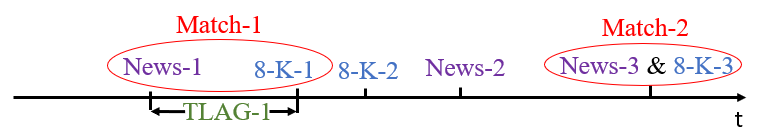
\includegraphics[scale=0.6]{../output/fig/fig1_matching.png}
	\end{center}
\end{figure}

Figuer 1 illustrates the 8-K sample matching process. We match every news day to its first posterior 8-K day, ignoring the successive 8-K days (if any) between two news days (Match-1), or in some cases the 8-K day coincides with news day (Match-2). TLAG is defined as the number of days elapsed between the news release date and 8-K filing date.

%%%%%%%%%%%%%% Figure 2: Sample Selection Process
% Table generated by Excel2LaTeX from sheet 'Fig2'
\begin{table}[htbp] \label{fig2}
  \centering
    \begin{tabular}{lr}
    \multicolumn{2}{c}{Figure 2: Sample Selection Process} \\
    \multicolumn{2}{c}{10-Q} \\
    Numer of observations: &  \\
    Retrieved from EDGAR & 575,579 \\
    After merging with COMP and CRSP data & 190,341 \\
    After merging with I\textbackslash{}B\textbackslash{}E\textbackslash{}S and segment data & 110,114 \\
    After dropping obs. with missing values in key variables and screening & \textbf{91,606} \\
      &  \\
    \multicolumn{2}{c}{8-K} \\
    Numer of observations: &  \\
    Retrieved from EDGAR & 1,489,626 \\
    After merging and matching with COMP and CRSP data & 390,698 \\
    After dropping obs. with missing values in key variables and screening & \textbf{244,401} \\
    After filtering obs. with TLAG smaller or equal to 4 (8-K restricted sample) & \textbf{61,443} \\
    \end{tabular}%
\end{table}%
 \label{fig2}

%%%%%%%%%%%%%% Figure 3: 8-K Item Distribution
\setcounter{figure}{2}
\begin{figure}[htbp]
	\begin{center}
		\caption{8-K Item Distribution} \label{fig3}
		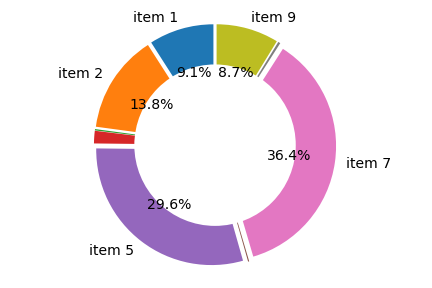
\includegraphics[scale=0.5]{../output/fig/fig3_8-K_before.png}
		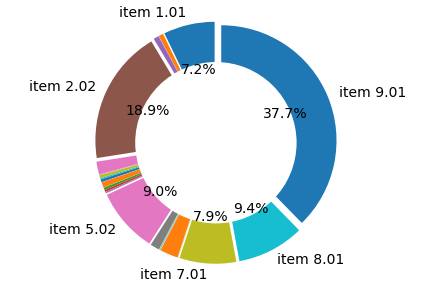
\includegraphics[scale=0.5]{../output/fig/fig3_8-K_after.png}
	\end{center}
\end{figure}

Figuer 3 illustrates the 8-K item distribution before (left) and after (right) August 23rd of 2004. Each share of pie chart shows the percentage of corporate events reported under each 8-K items. See 8-K item list in \hyperref[appd]{Appendix D}.

\newpage
%%%%%%%%%%%%%%%%%%%%%%%%%TABLE 1
\begin{table}[H]
	\centering
	\caption{Constituency Statute' Enactment Years (1975 - 2013)}
	\begin{tabular}{lrrrr}
		\toprule
		\toprule
		State & \multicolumn{1}{l}{Enactment date} & \multicolumn{1}{l}{Before} & \multicolumn{1}{l}{After} & \multicolumn{1}{l}{Total} \\
		\midrule
		AZ    & \multicolumn{1}{l}{07/22/1987} & 57    & 89    & 146 \\
		CT    & \multicolumn{1}{l}{06/07/1988} & 207   & 307   & 514 \\
		FL    & \multicolumn{1}{l}{06/27/1989} & 443   & 756   & 1199 \\
		GA    & \multicolumn{1}{l}{07/01/1989} & 292   & 518   & 810 \\
		HI    & \multicolumn{1}{l}{06/07/1989} & 39    & 52    & 91 \\
		IA    & \multicolumn{1}{l}{12/31/1989} & 95    & 130   & 225 \\
		ID    & \multicolumn{1}{l}{03/22/1988} & 13    & 26    & 39 \\
		IL    & \multicolumn{1}{l}{08/23/1985} & 139   & 277   & 416 \\
		IN    & \multicolumn{1}{l}{04/01/1986} & 261   & 519   & 780 \\
		KY    & \multicolumn{1}{l}{07/15/1988} & 49    & 74    & 123 \\
		LA    & \multicolumn{1}{l}{07/10/1988} & 77    & 114   & 191 \\
		MA    & \multicolumn{1}{l}{07/18/1989} & 687   & 969   & 1656 \\
		MD    & \multicolumn{1}{l}{06/01/1999} & 432   & 352   & 784 \\
		ME    & \multicolumn{1}{l}{09/19/1985} & 74    & 101   & 175 \\
		MN    & \multicolumn{1}{l}{06/01/1987} & 472   & 1,013 & 1485 \\
		MO    & \multicolumn{1}{l}{05/06/1986} & 165   & 306   & 471 \\
		MS    & \multicolumn{1}{l}{07/01/1990} & 2     & 23    & 25 \\
		NC    & \multicolumn{1}{l}{10/01/1993} & 262   & 250   & 512 \\
		NE    & \multicolumn{1}{l}{04/08/1988} & 50    & 32    & 82 \\
		NJ    & \multicolumn{1}{l}{02/04/1989} & 597   & 809   & 1406 \\
		NM    & \multicolumn{1}{l}{04/09/1987} & 30    & 47    & 77 \\
		NV    & \multicolumn{1}{l}{10/01/1991} & 419   & 564   & 983 \\
		NY    & \multicolumn{1}{l}{07/23/1987} & 1,351 & 1,999 & 3350 \\
		OH    & \multicolumn{1}{l}{10/10/1984} & 574   & 1,351 & 1925 \\
		OR    & \multicolumn{1}{l}{03/05/1989} & 134   & 223   & 357 \\
		PA    & \multicolumn{1}{l}{04/27/1990} & 883   & 1,144 & 2027 \\
		RI    & \multicolumn{1}{l}{07/03/1990} & 66    & 110   & 176 \\
		SD    & \multicolumn{1}{l}{07/01/1990} & 27    & 45    & 72 \\
		TN    & \multicolumn{1}{l}{03/11/1988} & 105   & 219   & 324 \\
		TX    & \multicolumn{1}{l}{01/01/2006} & 594   & 241   & 835 \\
		VA    & \multicolumn{1}{l}{03/31/1988} & 341   & 594   & 935 \\
		VT    & \multicolumn{1}{l}{04/16/1998} & 58    & 28    & 86 \\
		WI    & \multicolumn{1}{l}{06/13/1987} & 299   & 559   & 858 \\
		WY    & \multicolumn{1}{l}{01/01/1990} & 32    & 52    & 84 \\
		\midrule
		Total  &       & 9,326 & 13,893 & 23,219 \\
		\bottomrule
		\bottomrule
	\end{tabular}%
	\label{tab:addlabel}%
\end{table}%
\noindent This table presents the enactment dates and number of observations before and after enactment for 34 states out of 35 states that have adopted constituency statutes. North Dakota is excluded because of missing observations before or after law enactment date. Nebraska enacted constituency statute from 1988 to 1995 and from 2007 untill present.

%%%%%%%%%%%%%%%%%%%%%%%%%TABLE 2
\begin{table}[H]
	\centering
	\caption{Basu Summary Statistics (1975-2013)}
	Panel A. Firm-year Observations Before Constituency Statute Law Enactment (N=9,326)
	\begin{tabular}{lrrrrrrrrr}
		\toprule
		\toprule
		& \multicolumn{1}{l}{mean} & \multicolumn{1}{l}{median} & \multicolumn{1}{l}{std. dev.} & \multicolumn{1}{l}{max} & \multicolumn{1}{l}{min} & \multicolumn{1}{l}{p1} & \multicolumn{1}{l}{p25} & \multicolumn{1}{l}{p75} & \multicolumn{1}{l}{p99} \\
		\midrule
		EARN  & 0.088 & 0.098 & 0.151 & 0.378 & -1.034 & -0.524 & 0.049 & 0.163 & 0.378 \\
		RET   & 0.032 & 0.023 & 0.338 & 1.419 & -1.194 & -0.817 & -0.156 & 0.194 & 1.086 \\
		NEG   & 0.466 & 0.000 & 0.499 & 1.000 & 0.000 & 0.000 & 0.000 & 1.000 & 1.000 \\
		SIZE  & 4.310 & 4.144 & 1.953 & 10.388 & 0.623 & 0.623 & 2.841 & 5.636 & 9.264 \\
		BTM   & 0.882 & 0.773 & 0.576 & 3.256 & -0.980 & 0.054 & 0.481 & 1.153 & 3.010 \\
		LEV   & 0.692 & 0.348 & 0.972 & 7.773 & 0.000 & 0.000 & 0.093 & 0.934 & 5.024 \\
		\bottomrule
		\bottomrule
	\end{tabular}%
	\bigbreak
	Panel B. Firm-year Observations After Constituency Statutes Law Enactment (N=13,893)
	\begin{tabular}{lrrrrrrrrr}
		\toprule
		\toprule
		& \multicolumn{1}{l}{mean} & \multicolumn{1}{l}{median} & \multicolumn{1}{l}{std. dev} & \multicolumn{1}{l}{max} & \multicolumn{1}{l}{min} & \multicolumn{1}{l}{p1} & \multicolumn{1}{l}{p25} & \multicolumn{1}{l}{p75} & \multicolumn{1}{l}{p99} \\
		\midrule
		EARN  & 0.025 & 0.060 & 0.162 & 0.378 & -1.034 & -0.820 & 0.023 & 0.086 & 0.290 \\
		RET   & 0.013 & -0.005 & 0.351 & 1.419 & -1.194 & -0.924 & -0.173 & 0.180 & 1.156 \\
		NEG   & 0.509 & 1.000 & 0.500 & 1.000 & 0.000 & 0.000 & 0.000 & 1.000 & 1.000 \\
		SIZE  & 5.589 & 5.628 & 2.261 & 10.388 & 0.623 & 0.790 & 3.875 & 7.245 & 10.388 \\
		BTM   & 0.682 & 0.574 & 0.548 & 3.256 & -0.980 & -0.581 & 0.359 & 0.851 & 2.909 \\
		LEV   & 0.568 & 0.260 & 0.953 & 7.773 & 0.000 & 0.000 & 0.068 & 0.685 & 5.293 \\
		\bottomrule
		\bottomrule
	\end{tabular}%
	\bigbreak
	Panel C. Variable Difference Before and After Contituency Statute Law Enactment
	\begin{tabular}{lcc}
		\toprule
		\toprule
		& \multicolumn{1}{l}{mean difference} & \multicolumn{1}{l}{t-statistic} \\
		\midrule
		EARN  & -0.06*** & -29.76 \\
		RET   & -0.02*** & -4.18 \\
		NEG   & 0.04*** & 6.47 \\
		SIZE  & 1.28*** & 44.61 \\
		BTM   & -0.20*** & -26.79 \\
		LEV   & -0.12*** & -9.60 \\
		\bottomrule
		\bottomrule
	\end{tabular}%
\end{table}%
\noindent This table reports summary statistics for key variables used in Basu measure, separated into two time periods: before (Panel A) and after (Panel B) constituency statute enactment. Panel C demonstrates the differences in mean value between pre-enactment and post-enactment period for all key variables, and the significance of mean differences. EARN, RET, SIZE, BTM and LEV are winsorized at 1 and 99 percentiles. All variables are defined in Appendix B. *, **, and *** indicate significance at 10\%, 5\% and 1\% confidence level respectively.

%%%%%%%%%%%%%%%%%%%%%%%%%TABLE 3
\newgeometry{left=1cm, right=1cm, top=1cm, bottom=1.8cm}
\begin{landscape}
	\begin{table}[H]
		\centering
		\caption{Effect of Constituency Statue Enactments on Conservatism, Three Periods}
		$EARN_{i,t}=\alpha_i+\omega_t+\beta_1RET_{i,t}+\beta_2NEG_{i,t}+\beta_3RET_{i,t}\times NEG_{i,t}+\epsilon_{i,t}$ \qquad \qquad \qquad \qquad \qquad \qquad \qquad \qquad \qquad \qquad \qquad \qquad \qquad \qquad (1)
		
		$EARN_{i,t}=\alpha_i+\omega_t+\beta_1RET_{i,t}+\beta_2NEG_{i,t}+\beta_3RET_{i,t}\times NEG_{i,t}+POST_{i,t}\times (\beta_4+\beta_5RET_{i,t}+\beta_6NEG_{i,t}+\beta_7RET_{i,t}\times NEG_{i,t})+\epsilon_{i,t}$ (2)
		
		$\beta_j=\sum_{K}^{}\delta_{j,k}State_k+\sum_{M}^{}\theta_{j,m}Year_m \qquad j=1,2,3$ \qquad \qquad \qquad \qquad \qquad \qquad \qquad \qquad \qquad \qquad \qquad \qquad \qquad \qquad \qquad \qquad \qquad \quad (3)
		
		\begin{tabular}{lccccccc}
			\toprule
			\toprule
			Dependent Variable: EARN & Baseline Basu & \multicolumn{2}{c}{DiD: 1975-2013} & \multicolumn{2}{c}{1984-1992} & \multicolumn{2}{c}{1985-1990} \\
			& I     & II & III & IV & V& VI & VII \\
			&  &  & Incorp. = State &  & Incorp. = State&  & Incorp. = State\\
			\midrule
			RET   & 0.0603*** &       &       &       &       &       &  \\
			& 6.82  &       &       &       &       &       &  \\
			NEG   & 0.0019 &       &       &       &       &       &  \\
			& 0.70  &       &       &       &       &       &  \\
			\rowcolor[rgb]{ .851,  .851,  .851} RET $\times$ NEG & 0.1171*** &       &       &       &       &       &  \\
			\rowcolor[rgb]{ .851,  .851,  .851}       & 10.07 &       &       &       &       &       &  \\
			POST  &       & -0.006 & 0.0067 & -0.0204 & -0.0029 & -0.0098 & 0.0213 \\
			&       & -0.93 & 0.87  & -1.46 & -0.15 & -0.68 & 1.06 \\
			\rowcolor[rgb]{ .851,  .851,  .851} POST $\times$ RET &       & -0.0114 & -0.0334 & 0.0896 & 0.0508 & 0.0762 & -0.0312 \\
			\rowcolor[rgb]{ .851,  .851,  .851}       &       & -0.37 & -1.07 & 1.18  & 0.49  & 0.87  & -0.26 \\
			POST $\times$ NEG &       & 0.0035 & 0.0091 & -0.0012 & -0.0092 & -0.0133 & -0.0377 \\
			&       & 0.35  & 0.90  & -0.07 & -0.45 & -0.47 & -1.38 \\
			\rowcolor[rgb]{ .851,  .851,  .851} POST $\times$ RET $\times$ NEG &       & 0.1041* & 0.1961*** & 0.0109 & 0.0055 & 0.0421 & 0.0833 \\
			\rowcolor[rgb]{ .851,  .851,  .851}       &       & 2.05  & 4.37  & 0.09  & 0.04  & 0.36  & 0.60 \\
			Constant & 0.1597*** & 0.0644** & 0.0571** & 0.0277 & 0.0171 & 0.0442** & 0.0127 \\
			& 17.27 & 3.45  & 2.77  & 1.53  & 0.87  & 2.80 & 0.64 \\
			Year Fixed Effects (Main) & YES   & YES   & YES   & YES   & YES   & YES   & YES \\
			Firm Fixed Effects (Main) & YES   & YES   & YES   & YES   & YES   & YES   & YES \\
			Year Fixed Effects (Basu Coefficients) & NO    & YES   & YES   & YES   & YES   & YES   & YES \\
			State Fixed Effects (Basu Coefficients) & NO    & YES   & YES   & YES   & YES   & YES   & YES \\
			S.E. Clustered by States & YES   & YES   & YES   & YES   & YES   & YES   & YES \\
			Observations  & 23,219 &                  23,219  &                  17,347  &                     7,202  &                     5,314  &                     4,806  &                    3,514  \\
			Adj. R-square & 0.2970 & 0.3108 & 0.3229 & 0.3645 & 0.3716 & 0.3916 & 0.3950 \\
			\bottomrule
			\bottomrule
		\end{tabular}%
	\end{table}%
	
	\noindent This table reports results of baseline Basu measure (Equation 1) over full sample period (Column I), and DiD results (Equation 2 and 3) in three sample periods: 1975 - 2013 (Column II, III), 1984 - 1992 (Column IV, V) and 1985 - 1990 (Column VI, VII). Column III, Column V and Column VII show the DiD results using only firms that headquarter in their state of incorporation. All variables are defined in Appendix B. EARN and RET are winsorized at 1 and 99 percentiles. All regressions control for firm and year fixed effects. DiD regressions control for Basu coefficient fixed effects. Standard errors are clustered at state of incorporation level. %The Basu coefficient fixed effects absorb slope coefficients in baseline Basu model so they are omitted.  *, **, and *** indicate significance at 10\%, 5\% and 1\% confidence level respectively. T-statistics are reported below coefficients.
	
\end{landscape}
\restoregeometry

%\begin{table}[H]
%\centering
%\caption{Basu Measure of Conditional Conservatism}
%$EARN_{i,t}=\alpha_i+\omega_t+\beta_1RET_{i,t}+\beta_2NEG_{i,t}+\beta_3RET_{i,t}\times NEG_{i,t}+\epsilon_{i,t}$
%\begin{tabular}{lccc}
%\toprule
%\toprule
%Dep. Var. EARN & Prediction & 1975-2013 & 1985-1990 \\
%\midrule
%Constant &       & 0.1597*** & 0.0681*** \\
%&       & 17.27 & 12.54 \\
%RET   &       & 0.0603*** & 0.0793** \\
%&       & 6.82  & 2.84 \\
%NEG   &       & 0.0019 & 0.0087 \\
%&       & 0.70  & 1.21 \\
%\rowcolor[rgb]{ .851,  .851,  .851} RET $\times$ NEG & (+)   & 0.1171*** & 0.0932* \\
%\rowcolor[rgb]{ .851,  .851,  .851}       &       & 10.07 & 2.71 \\
%Year Fixed Effects  &       & YES   & YES \\
%Firm Fixed Effects &       & YES   & YES \\
%S.E. Clustered by States &       & YES   & YES \\
%Observations     &       & 23,219 & 4,806 \\
%Adj. R-square &       & 0.2970 & 0.3781 \\
%\bottomrule
%\bottomrule
%\end{tabular}%
%\end{table}%
%
%%%%%%%%%%%%%%%%TABLE 4
%\begin{table}[H]
%\centering
%\caption{DiD: Effect of Constituency Statue Enactments on Conservatism, Two Periods}
%
%$EARN_{i,t}=\alpha_i+\omega_t+\beta_1RET_{i,t}+\beta_2NEG_{i,t}+\beta_3RET_{i,t}\times NEG_{i,t}+POST_{i,t}\times (\beta_4+\beta_5RET_{i,t}+\beta_6NEG_{i,t}+\beta_7RET_{i,t}\times NEG_{i,t})+\epsilon_{i,t}$
%
%\begin{tabular}{lcccc}
%\toprule
%\toprule
%Dep. Var. EARN & \multicolumn{2}{c}{1975-2013} & \multicolumn{2}{c}{1985-1990} \\
%& I & II& III & IV\\
%& Full & Incorp.=State & Full & Incorp.=State\\
%\midrule
%POST  & -0.006 & 0.0067 & -0.0098 & 0.0213 \\
%& -0.93 & 0.87  & -0.68 & 1.06 \\
%\rowcolor[rgb]{ .851,  .851,  .851} POST $\times$ RET & -0.0114 & -0.0334 & 0.0762 & -0.0312 \\
%\rowcolor[rgb]{ .851,  .851,  .851}       & -0.37 & -1.07 & 0.87  & -0.26 \\
%POST $\times$ NEG & 0.0035 & 0.0091 & -0.0133 & -0.0377 \\
%& 0.35  & 0.90  & -0.47 & -1.38 \\
%\rowcolor[rgb]{ .851,  .851,  .851} POST $\times$ RET $\times$ NEG & 0.1041* & 0.1961*** & 0.0421 & 0.0833 \\
%\rowcolor[rgb]{ .851,  .851,  .851}       & 2.05  & 4.37  & 0.36  & 0.60 \\
%Constant & 0.0644** & 0.0571** & 0.0442** & 0.0127 \\
%& 3.45  & 2.77  & 2.80   & 0.64 \\
%Year Fixed Effects (Main) & YES   & YES   & YES   & YES \\
%Firm Fixed Effects (Main) & YES   & YES   & YES   & YES \\
%Year Fixed Effects (Basu Coefficients) & YES   & YES   & YES   & YES \\
%State Fixed Effects (Basu Coefficients) & YES   & YES   & YES   & YES \\
%S.E. Clustered by States & YES   & YES   & YES   & YES \\
%Observations  &                  23,219  &                  17,347  &                     4,806  &                     3,514  \\
%Adj. R-square & 0.3108 & 0.3229 & 0.3916 & 0.3950 \\
%\bottomrule
%\bottomrule
%\end{tabular}%
%\end{table}%

%%%%%%%%%%TABLE 4
\begin{landscape}
	\begin{table}[H]
		\centering
		\caption{DiD: Effect of Constituency Statue Enactments on Conservatism, Rolling Windows}
		$EARN_{i,t}=\alpha_i+\omega_t+\beta_1RET_{i,t}+\beta_2NEG_{i,t}+\beta_3RET_{i,t}\times NEG_{i,t}+Dummy_{i,t}\times (\beta_4+\beta_5RET_{i,t}+\beta_6NEG_{i,t}+\beta_7RET_{i,t}\times NEG_{i,t})+\epsilon_{i,t}$
		\begin{tabular}{lcccccc}
			\toprule
			\toprule
			Dep. Var. EARN & I & II & III & IV & V & VI \\
			& -1/+1 &  -1/+1 & -2/+2 & -2/+2 & -3/+3 & -3/+3 \\
			& Full & Incorp.= State & Full & Incorp.= State & Full & Incorp.= State \\
			\midrule
			\rowcolor[rgb]{ .906,  .902,  .902} Dummy $\times$ RET$\times$ NEG & 0.1717 & 0.1257 & 0.1622* & 0.1291 & 0.1358** & 0.1266* \\
			& 2.02  & 1.26  & 2.24  & 1.65  & 2.93  & 2.71 \\
			Dummy & -0.0149 & 0.0124 & 0.0187 & 0.0396 & 0.0005 & 0.016 \\
			& -0.92 & 0.71 & 1.01 & 1.61 & 0.04 & 0.94 \\
			Dummy$\times$RET & 0.024 & -0.0052 & 0.0056 & 0.0015 & -0.0079 & -0.0131 \\
			& 0.47 & -0.08 & 0.16 & 0.03 & -0.29 & -0.32 \\
			Dummy$\times$NEG & -0.0042 & -0.0269 & 0.0085 & -0.0035 & 0.007 & -0.0005 \\
			& -0.15 & -0.68 & 0.68 & -0.23 & 0.59 & -0.03 \\
			Constant & 0.0235 & 0.0394* & 0.0900*** & 0.1014*** & 0.1364*** & 0.1368*** \\
			& 1.42 & 2.29 & 4.12 & 4.74 & 11.45 & 10.80 \\
			Year Fixed Effects (Main) & Yes & Yes & Yes & Yes & Yes & Yes \\
			Firm Fixed Effects (Main) & Yes & Yes & Yes & Yes & Yes & Yes \\
			S.E. Clustered by States & Yes & Yes & Yes & Yes & Yes & Yes \\
			Observations & 2,220 & 1,612 & 4,241 & 3,093 & 6,134 & 4,492 \\
			Adj. R-squared & 0.4286 & 0.4169 & 0.3923 & 0.3686 & 0.3655 & 0.3543 \\
			\bottomrule
			\bottomrule
		\end{tabular}%
		\label{tab:addlabel}%
	\end{table}%
	
	\noindent This table reports results of rolling window analysis of conservatism (measured by Basu model) in three subsamples that consist of firm-year observations within one-year (-1/+1), two-years (-2/+2) and three-years (-3/+3) window before and after constituency statute enactments in all states that have adopted the law as of 2013. Column II, Column IV and Column VI show the rolling window results using only firms that headquarter in their state of incorporation. \textit{Dummy} is an indicator variable that takes 1 if this firm-year observation is recorded after law enactment, and 0 if before law enactment. The rest of variables are defined in Appendix B. EARN and RET are winsorized at 1 and 99 percentiles. All regressions control for year and firm fixed effects. Standard errors are clustered at state of incorporation level. *, **, and *** indicate significance at 10\%, 5\% and 1\% confidence level, respectively. t-statistics are reported below coefficients.
\end{landscape}

%%%%%%%%%%%%%%%%%%%%%%TABLE 5
\newgeometry{left=1cm, right=1cm, top=1.7cm, bottom=2cm}
\begin{table}[H]
	\centering
	\caption{Mechanism (1975 - 2013)}                                                 
	\begin{flushleft}
		$EARN_{i,t}=\alpha_i+\omega_t+\beta_1RET_{i,t}+\beta_2NEG_{i,t}+\beta_3RET_{i,t}\times NEG_{i,t}+POST_{i,t}\times (\beta_4+\beta_5RET_{i,t}+\beta_6NEG_{i,t}+\beta_7RET_{i,t}\times NEG_{i,t})+MEC\times(\beta_8RET_{i,t}+\beta_9NEG_{i,t}+\beta_{10}REG_{i,t}\times NEG_{i,t})+MEC\times POST_{i,t}\times (\beta_{11}+\beta_{12}RET_{i,t}+\beta_{13}NEG_{i,t}+\beta_{14}RET_{i,t}\times NEG_{i,t})+\epsilon_{i,t}$ \qquad \qquad \qquad \qquad \qquad \qquad \qquad \qquad \qquad \qquad \qquad(4)
	\end{flushleft}
	\begin{tabular}{lccc}
		\toprule
		\toprule
		Dep. Var. EARN & DCD1 & DCD2 & MA \\
		\midrule
		POST  & 0.0003 & -0.0056 & -0.0160* \\
		& 0.05  & -0.86 & -2.15 \\
		POST$\times$ RET & 0.0112 & -0.0150 & 0.0254 \\
		& 0.38  & -0.47 & 0.81 \\
		POST$\times$NEG & 0.0000 & -0.0022 & 0.0129 \\
		& 0.00  & -0.22 & 1.13 \\
		\rowcolor[rgb]{ .851,  .851,  .851} POST$\times$RET$\times$NEG & -0.0657 & 0.0316 & 0.0709 \\
		\rowcolor[rgb]{ .851,  .851,  .851}       & -1.43 & 0.61  & 1.23 \\
		MEC$\times$RET & 0.0103 & 0.0158 & 0.7419*** \\
		& 0.59  & 1.84  & 4.53 \\
		MEC$\times$NEG & -0.0039 & -0.0024 & 0.1201** \\
		& -0.36 & -0.37 & 2.98 \\
		MEC$\times$RET$\times$NEG & -0.1059* & -0.0700* & -1.5956*** \\
		& -2.46 & -2.34 & -4.21 \\
		MEC$\times$POST & -0.0100 & -0.0220* & 0.1592*** \\
		& -1.31 & -2.47 & 6.14 \\
		MEC$\times$POST$\times$RET & -0.0581* & -0.0562*** & -0.7353*** \\
		& -2.33 & -3.61 & -3.84 \\
		MEC$\times$POST$\times$NEG & 0.0023 & -0.0105 & -0.1559** \\
		& 0.18  & -0.79 & -2.80 \\
		\rowcolor[rgb]{ .851,  .851,  .851} MEC$\times$POST$\times$RET$\times$NEG & 0.2854*** & 0.1751*** & 1.1218* \\
		\rowcolor[rgb]{ .851,  .851,  .851}       & 7.74  & 4.90  & 2.65 \\
		Constant & 0.0609** & 0.0599** & 0.0742*** \\
		& 3.17  & 2.88  & 3.73 \\
		Year Fixed Effects (Main) & YES   & YES   & YES \\
		Firm Fixed Effects (Main) & YES   & YES   & YES \\
		Year Fixed Effects (Basu Coefficients) & YES   & YES   & YES \\
		State Fixed Effects (Basu Coefficients) & YES   & YES   & YES \\
		S.E. Clustered by States & YES   & YES   & YES \\
		Observations    & 23219 & 23219 & 18277 \\
		Adj. R-squared & 0.318 & 0.3334 & 0.2836 \\
		\bottomrule
		\bottomrule
	\end{tabular}%
\end{table}%
\noindent This table reports results of Equation (4): earnings on baseline Basu factors (i.e., NEG, RET, NEG $\times$ RET) and their interactions with POST dummy and three mechanism variables (DCD1, DCD2 and MA). All variables are defined in Appendix B. EARN and RET are winsorized at 1 and 99 percentiles. All regressions control for main firm and year fixed effects and Basu coefficient fixed effects. Standard errors are clustered at state of incorporation level. The Basu coefficient fixed effects absorb slope coefficients in baseline Basu model so they are omitted.  *, **, and *** indicate significance at 10\%, 5\% and 1\% confidence level respectively. T-statistics are reported below coefficients.

\restoregeometry

%%%%%%%%%%%%%%%%%%%TABLE 6
\begin{table}[H]
	\centering
	\caption{KLD Indexes (1995 - 2013)}
	
	Panel A. KLD Summary Statistics
	\begin{tabular}{lrrrrrrrrrr}
		\toprule
		\toprule
		& \multicolumn{1}{l}{N} & \multicolumn{1}{l}{mean} & \multicolumn{1}{l}{median} & \multicolumn{1}{l}{std. dev.} & \multicolumn{1}{l}{max} & \multicolumn{1}{l}{min} & \multicolumn{1}{l}{p1} & \multicolumn{1}{l}{p25} & \multicolumn{1}{l}{p75} & \multicolumn{1}{l}{p99} \\
		\midrule
		KLD\_STR & 12341 & 0.476 & 0     & 1.060 & 12    & 0     & 0     & 0     & 1     & 5 \\
		KLD\_CON & 13922 & 1.011 & 1     & 1.518 & 13    & 0     & 0     & 0     & 1     & 7 \\
		KLD\_TOTAL & 12341 & -0.515 & 0     & 1.403 & 8     & -9    & -5    & -1    & 0     & 3 \\
		Enviroment & 15800 & 0.137 & 0     & 0.427 & 4     & 0     & 0     & 0     & 0     & 2 \\
		Community & 15624 & 0.147 & 0     & 0.476 & 5     & 0     & 0     & 0     & 0     & 2 \\
		Product & 15624 & 0.071 & 0     & 0.272 & 3     & 0     & 0     & 0     & 0     & 1 \\
		Emloyee relation & 12341 & 0.241 & 0     & 0.571 & 5     & 0     & 0     & 0     & 0     & 2 \\
		Human rights & 12986 & 0.003 & 0     & 0.054 & 1     & 0     & 0     & 0     & 0     & 0 \\
		\bottomrule
		\bottomrule
	\end{tabular}%
	
	\bigbreak
	Panel B. KLD Indexes Correlation Matrix
	\begin{tabular}{lrrrrrrrr}
		\toprule
		\toprule
		& KLD\_STR & KLD\_CON & KLD\_TOTAL & Env. & Com. & Prod. & Emp. & Hum.\\
		\midrule
		KLD\_STR & 1.000 &       &       &       &       &       &       &  \\
		KLD\_CON & 0.425 & 1.000 &       &       &       &       &       &  \\
		KLD\_TOTAL & 0.309 & -0.730 & 1.000 &       &       &       &       &  \\
		Enviroment & 0.655 & 0.331 & 0.122 & 1.000 &       &       &       &  \\
		Community & 0.662 & 0.305 & 0.174 & 0.264 & 1.000 &       &       &  \\
		Product & 0.500 & 0.116 & 0.235 & 0.204 & 0.149 & 1.000 &       &  \\
		Employee relation & 0.801 & 0.307 & 0.282 & 0.306 & 0.287 & 0.256 & 1.000 &  \\
		Human rights & 0.145 & 0.043 & 0.062 & 0.023 & 0.117 & 0.031 & 0.064 & 1.000 \\
		\bottomrule
		\bottomrule
	\end{tabular}%
\end{table}%
\noindent This table reports summary statistics (Panel A) and correlation matrix (Panel B) of KLD indexes from 1995 to 2013. All indexes are defined in Appendix C.

%%%%%%%%%%%%%%%%%%TABLE 7
\newgeometry{left=1cm, right=1cm, top=2cm, bottom=2cm}
\begin{landscape}
	\begin{table}[H]
		\centering
		\caption{Association between KLD Indexes and Conservatism , Measured by C\textunderscore Score (1995 - 2013)}
		
		$Conservatism_{i,t}=a_i+b_t+c\times KLD\textunderscore INDEX+d\times X_{i,t}+\epsilon_{i,t}$ \qquad (8)
		
		\begin{tabular}{lccccccc}
			\toprule
			\toprule
			Dependent Variable: C\_Score & I     & II    & III   & IV    & V     & VI    & VII \\
			\midrule
			KLD\_STR & \cellcolor[rgb]{ .906,  .902,  .902}0.0030*** & \cellcolor[rgb]{ .906,  .902,  .902} & \cellcolor[rgb]{ .906,  .902,  .902} & \cellcolor[rgb]{ .906,  .902,  .902} & \cellcolor[rgb]{ .906,  .902,  .902} & \cellcolor[rgb]{ .906,  .902,  .902} & \cellcolor[rgb]{ .906,  .902,  .902}              \\
			& \cellcolor[rgb]{ .906,  .902,  .902}4.95 & \cellcolor[rgb]{ .906,  .902,  .902} & \cellcolor[rgb]{ .906,  .902,  .902} & \cellcolor[rgb]{ .906,  .902,  .902} & \cellcolor[rgb]{ .906,  .902,  .902} & \cellcolor[rgb]{ .906,  .902,  .902} & \cellcolor[rgb]{ .906,  .902,  .902} \\
			KLD\textunderscore TOTAL   & \cellcolor[rgb]{ .906,  .902,  .902} & \cellcolor[rgb]{ .906,  .902,  .902}-0.0011* & \cellcolor[rgb]{ .906,  .902,  .902} & \cellcolor[rgb]{ .906,  .902,  .902} & \cellcolor[rgb]{ .906,  .902,  .902} & \cellcolor[rgb]{ .906,  .902,  .902} & \cellcolor[rgb]{ .906,  .902,  .902} \\
			& \cellcolor[rgb]{ .906,  .902,  .902} & \cellcolor[rgb]{ .906,  .902,  .902}-2.07 & \cellcolor[rgb]{ .906,  .902,  .902} & \cellcolor[rgb]{ .906,  .902,  .902} & \cellcolor[rgb]{ .906,  .902,  .902} & \cellcolor[rgb]{ .906,  .902,  .902} & \cellcolor[rgb]{ .906,  .902,  .902} \\
			Environment & \cellcolor[rgb]{ .906,  .902,  .902} & \cellcolor[rgb]{ .906,  .902,  .902} & \cellcolor[rgb]{ .906,  .902,  .902}-0.0019 & \cellcolor[rgb]{ .906,  .902,  .902} & \cellcolor[rgb]{ .906,  .902,  .902} & \cellcolor[rgb]{ .906,  .902,  .902} & \cellcolor[rgb]{ .906,  .902,  .902} \\
			& \cellcolor[rgb]{ .906,  .902,  .902} & \cellcolor[rgb]{ .906,  .902,  .902} & \cellcolor[rgb]{ .906,  .902,  .902}-1.93 & \cellcolor[rgb]{ .906,  .902,  .902} & \cellcolor[rgb]{ .906,  .902,  .902} & \cellcolor[rgb]{ .906,  .902,  .902} & \cellcolor[rgb]{ .906,  .902,  .902} \\
			Community & \cellcolor[rgb]{ .906,  .902,  .902} & \cellcolor[rgb]{ .906,  .902,  .902} & \cellcolor[rgb]{ .906,  .902,  .902} & \cellcolor[rgb]{ .906,  .902,  .902}-0.0020* & \cellcolor[rgb]{ .906,  .902,  .902} & \cellcolor[rgb]{ .906,  .902,  .902} & \cellcolor[rgb]{ .906,  .902,  .902} \\
			& \cellcolor[rgb]{ .906,  .902,  .902} & \cellcolor[rgb]{ .906,  .902,  .902} & \cellcolor[rgb]{ .906,  .902,  .902} & \cellcolor[rgb]{ .906,  .902,  .902}-2.45 & \cellcolor[rgb]{ .906,  .902,  .902} & \cellcolor[rgb]{ .906,  .902,  .902} & \cellcolor[rgb]{ .906,  .902,  .902} \\
			Product & \cellcolor[rgb]{ .906,  .902,  .902} & \cellcolor[rgb]{ .906,  .902,  .902} & \cellcolor[rgb]{ .906,  .902,  .902} & \cellcolor[rgb]{ .906,  .902,  .902} & \cellcolor[rgb]{ .906,  .902,  .902}0.0060* & \cellcolor[rgb]{ .906,  .902,  .902} & \cellcolor[rgb]{ .906,  .902,  .902} \\
			& \cellcolor[rgb]{ .906,  .902,  .902} & \cellcolor[rgb]{ .906,  .902,  .902} & \cellcolor[rgb]{ .906,  .902,  .902} & \cellcolor[rgb]{ .906,  .902,  .902} & \cellcolor[rgb]{ .906,  .902,  .902}2.42 & \cellcolor[rgb]{ .906,  .902,  .902} & \cellcolor[rgb]{ .906,  .902,  .902} \\
			Employee Relation & \cellcolor[rgb]{ .906,  .902,  .902} & \cellcolor[rgb]{ .906,  .902,  .902} & \cellcolor[rgb]{ .906,  .902,  .902} & \cellcolor[rgb]{ .906,  .902,  .902} & \cellcolor[rgb]{ .906,  .902,  .902} & \cellcolor[rgb]{ .906,  .902,  .902}0.0028** & \cellcolor[rgb]{ .906,  .902,  .902} \\
			& \cellcolor[rgb]{ .906,  .902,  .902} & \cellcolor[rgb]{ .906,  .902,  .902} & \cellcolor[rgb]{ .906,  .902,  .902} & \cellcolor[rgb]{ .906,  .902,  .902} & \cellcolor[rgb]{ .906,  .902,  .902} & \cellcolor[rgb]{ .906,  .902,  .902}3.47 & \cellcolor[rgb]{ .906,  .902,  .902} \\
			Human Rights & \cellcolor[rgb]{ .906,  .902,  .902} & \cellcolor[rgb]{ .906,  .902,  .902} & \cellcolor[rgb]{ .906,  .902,  .902} & \cellcolor[rgb]{ .906,  .902,  .902} & \cellcolor[rgb]{ .906,  .902,  .902} & \cellcolor[rgb]{ .906,  .902,  .902} & \cellcolor[rgb]{ .906,  .902,  .902}-0.0059 \\
			& \cellcolor[rgb]{ .906,  .902,  .902} & \cellcolor[rgb]{ .906,  .902,  .902} & \cellcolor[rgb]{ .906,  .902,  .902} & \cellcolor[rgb]{ .906,  .902,  .902} & \cellcolor[rgb]{ .906,  .902,  .902} & \cellcolor[rgb]{ .906,  .902,  .902} & \cellcolor[rgb]{ .906,  .902,  .902}-0.80 \\
			SIZE  & -0.0094*** & -0.0093*** & -0.0114*** & -0.0108*** & -0.0108*** & -0.0095*** & -0.0102*** \\
			& -8.41 & -8.11 & -9.34 & -8.64 & -8.74 & -8.18 & -8.77 \\
			MTB   & 0.0052*** & 0.0052*** & 0.0055*** & 0.0053*** & 0.0054*** & 0.0052*** & 0.0058*** \\
			& 26.27 & 26.17 & 15.15 & 18.34 & 18.19 & 26.28 & 28.29 \\
			LEV   & 0.061*** & 0.061*** & 0.0576*** & 0.0574*** & 0.0574*** & 0.0610*** & 0.0580*** \\
			& 24.19 & 23.88 & 26.32 & 26.55 & 26.48 & 23.99 & 22.85 \\
			Constant & 0.2287*** & 0.2287*** & 0.0176 & 0.0148 & 0.0136 & 0.2295*** & 0.1523*** \\
			& 30.31 & 29.85 & 1.96  & 1.57  & 1.43  & 29.76 & 22.15 \\
			Year fixed effects & YES   & YES   & YES   & YES   & YES   & YES   & YES \\
			Firm Fixed Effects & YES   & YES   & YES   & YES   & YES   & YES   & YES \\
			S.E. Clustered by States & YES   & YES   & YES   & YES   & YES   & YES   & YES \\
			Observations    & 10483 & 10483 & 13920 & 13742 & 13742 & 10483 & 11087 \\
			Adj. R-square & 0.7778 & 0.7776 & 0.778 & 0.7752 & 0.7753 & 0.7776 & 0.7708 \\
			\bottomrule
			\bottomrule
		\end{tabular}%
		\label{tab:addlabel}%
	\end{table}%
	
	\noindent This table reports results of Equation (8): OLS regression model of conservatism (measured by C\textunderscore Score) on KLD indexes. All KLD indexes are defined in Appendix c. All regressions control for firm and year fixed effects. Standard errors are clustered at state of incorporation level. *, **, and *** indicate significance at 10\%, 5\% and 1\% confidence level respectively. T-statistics are reported below coefficients.
	
\end{landscape}
\restoregeometry

%%%%%%%%%%%TABLE 8
\begin{table}[H]
	\centering
	\caption{DiD: Effect  of Constituency Statute Enactments on C\textunderscore Score, Three Periods}
	$Conservatism_{i,t}=a_i+b_t+c\times POST_{i,t}+d\times X_{i,t}+\epsilon_{i,t}$ \qquad (9)
	\begin{tabular}{lccc}
		\toprule
		\toprule
		Dep. Var. C\_Score & 1975 - 2013 & 1984 - 1992 & 1985 - 1990 \\
		& I & II & III \\
		\midrule
		\rowcolor[rgb]{ .906,  .902,  .902} POST  & 0.0046 & 0.0073* & 0.0112* \\
		\rowcolor[rgb]{ .906,  .902,  .902}       & 1.56  & 2.17  & 2.51 \\
		SIZE  & -0.0150*** & -0.0355*** & -0.0441*** \\
		& -8.27 & -12.94 & -8.83 \\
		MTB   & -0.0018 & -0.0051*** & -0.0044* \\
		& -1.64 & -5.83 & -2.73 \\
		LEV   & 0.0633*** & 0.0329*** & 0.0218*** \\
		& 23.07 & 10.45 & 3.99 \\
		Constant & 0.0824*** & 0.1695*** & 0.2749*** \\
		& 8.98  & 12.68 & 11.41 \\
		Year Fixed Effects & YES   & YES   & YES \\
		Firm Fixed Effects & YES   & YES   & YES \\
		S.E. Clustered by States & YES   & YES   & YES \\
		Observations  & 22570 & 6965  & 4644 \\
		Adj. R-square & 0.5016 & 0.5482 & 0.5194 \\
		\bottomrule
		\bottomrule
	\end{tabular}%
\end{table}%

\noindent This table reports DiD regression (Equation 9) results in three sample periods: 1975 - 2013 (Column I), 1984 - 1992 (Column II) and 1985 - 1990 (Column III). All variables are defined in Appendix B. SIZE, MTB and LEV are winsorized at 1 and 99 percentiles. All regressions control for firm and year fixed effects. Standard errors are clustered at state of incorporation level. *, **, and *** indicate significance at 10\%, 5\% and 1\% confidence level respectively. T-statistics are reported below coefficients.

%%%%%%%%%%%%TABLE 9
\begin{table}[H]
	\centering
	\caption{DiD: Effect of Constituency Statute Enactments on C\textunderscore Score, Rolling Windows}
	$Conservatism_{i,t}=a_i+b_t+c\times Dummy_{i,t}+d\times X_{i,t}+\epsilon_{i,t}$
	\begin{tabular}{lccc}
		\toprule
		\toprule
		Dep. Var. C\_SCORE & I & II & III \\
		\multicolumn{1}{r}{} & -1/+1 & -2/+2 & -3/+3 \\
		\midrule
		\rowcolor[rgb]{ .906,  .902,  .902} Dummy & 0.0223*** & 0.011 & 0.0083 \\
		\rowcolor[rgb]{ .906,  .902,  .902} & 5.89  & 1.09  & 1.36 \\
		SIZE  & -0.0387** & -0.0303***& -0.0318*** \\
		& -3.03 & -5.74 & -6.92 \\
		MTB   & -0.0032 & -0.0049** & -0.0041** \\
		& -1.02 & -3.26 & -3.56 \\
		LEV   & 0.0164 & 0.0319** & 0.0341*** \\
		& 0.74  & 2.92  & 5.13 \\
		Constant & 0.2184*** & 0.2130*** & 0.1846*** \\
		& 3.80  & 8.03  & 8.11 \\
		Year Fixed Effects & Yes & Yes & Yes \\
		Firm Fixed Effects & Yes & Yes & Yes \\
		S.E. Clustered by States & Yes & Yes & Yes \\
		Observations & 2,144 & 4,105 & 5,941 \\
		Adj. R-squared & 0.6858 & 0.7176 & 0.6896 \\
		\bottomrule
		\bottomrule
	\end{tabular}%
\end{table}%
\noindent This table reports results of rolling window analysis of conservatism (measured by C\textunderscore Score) in three subsamples that consist of firm-year observations within one-year (-1/+1), two-years (-2/+2) and three-years (-3/+3) window before and after constituency statute enactments in all states that have adopted the law as of 2013. \textit{Dummy} is an indicator variable that takes 1 if this firm-year observation is recorded after law enactment, and 0 if before law enactment. The rest of variables are defined in Appendix B. SIZE, MTB and LEV are winsorized at 1 and 99 percentiles. All regressions control for year and firm fixed effects. Standard errors are clustered at state of incorporation level. *, **, and *** indicate significance at 10\%, 5\% and 1\% confidence level, respectively. t-statistics are reported below coefficients.

\newpage
\section*{Appendix}
\subsection*{Appendix A: 10-Q and 8-K parsing}
\label{appa}
We develop a Python program to automatically parse, process and retrieve 10-K and 8-K filings from EDGAR database. Our algorithm consists of the following steps:

1. Download all quarterly master indexes from EDGAR using \textit{python-edgar}\footnote{Python-edgar package documentation available at \url{https://github.com/edouardswiac/python-edgar/blob/master/README.md}} package.

2. Filter all 10-Q and 8-K filings\footnote{Our analysis exclude amendments such as 10-Q/A and 8-K/A} from EDGAR master index files and obtain url of the \textit{filing detail} webpage\footnote{One example of filing detail webpage is available at \url{https://www.sec.gov/Archives/edgar/data/320193/000032019320000050/0000320193-20-000050-index.html}} for each of the 10-Q and 8-K filings. 

3. Extract (a) identification information\footnote{For example cik, accession number, reporting period, filing date and 8-K items etc.} and (b) url of report in HTM/TXT format\footnote{One example of report in HTM format is available at \url{https://www.sec.gov/Archives/edgar/data/320193/000032019320000050/a8-kq220203282020.htm}. We first search for url of main report in HTM format. If HTM format main report is not available, then we extract the url of TXT format full report. Each EDGAR filing can be accessed in three formats at maximum: regular text (*.txt), web pages (*.htm) and eXtensible Business Reporting Language, also known as XBRL (*.xml). Early filings in EDGAR are only in TXT format. Later filings extend to HTM format, and in 2009 SEC adopted the XBRL for all corporate filings \cite{secFinalRuleInteractive2009}. Therefore, current existing EDGAR filings all contain a TXT file, and depending on their filing date and company reporting policy they may or may not contain HTM or XML files. Normally all filings in XML format are also available in HTM format. We manually checked 100 random filings that are in XML format, and all of them are also available in HTM format with the same content. The TXT files usually contain not only the main report, but also all other additional filing materials (if any) such as graphics, exhibits and press release etc. However, the HTM files only contain the main report. We mainly focus on HTM files other than TXT files because the former naturally filters out less relevant information, and provides a cleaner textual content of the essential information. XML files are not parsed due to low tractability. } from the \textit{filing detail} webpage for each of the 10-Q and 8-K filings. 

4. Parse and cleanse\footnote{Cleansing steps are: (a) delete nondisplay section; (b) delete all tables that contains more than 4 numbers; and (c) delete all HTML tags} all 10-Q and 8-K filings with url of HTM/TXT format report, using \textit{beautiful soup}\footnote{Beautiful soup package documentation available at \url{https://www.crummy.com/software/BeautifulSoup/bs4/doc/}} package. 

5. Save all clean 10-Q and 8-K filings to local device. 

6. Perform word count on clean 10-Q and 8-K filings using LM dictionary.\footnote{LM dictionary available at \url{https://sraf.nd.edu/textual-analysis/resources/\#LM\%20Sentiment\%20Word\%20Lists}}

All Python scripts and data are available online via \url{https://github.com/fengzhi22/narrative_conservatism}.

\subsection*{Appendix B: Textual Variable Definition}
\label{appb}
\begin{table}[H]
	\centering
	\begin{tabular}{lp{15cm}p{15cm}}
		\textbf{Variable} & \textbf{Definition} \\
		NW & Number of words, defined as the natural logarithm of one plus the count of total words (nw)\\
		nw & Raw count of total words\\
		TONE & Tone, defined as number of net positive words per thousand total words, calculated as total number of positive words minus the sum of total number of negative words and total number of negations, and multiply the previous result by one thousand\\
		TLAG & Time lag, defined as number of days elapsed between the news release date (CRSP entry date) and document filing date (EDGAR filing date)\\
		ABTONE & Abnormal tone, calculated as the residual of the cross-sectional expected tone model (Equation 3)\\
		N8K & Number of 8-Ks reported in one day\\
		NITEM & Number of 8-K items reported in one day\\
		
	\end{tabular}%
\end{table}%

\subsection*{Appendix C: Financial Variable Definition}
\label{appc}
\begin{table}[H]
	\centering
	\begin{tabular}{lp{15cm}p{15cm}}
		\textbf{Variable} & \textbf{Definition} \\
		
		EARN & Quarterly earnings, defined as quarterly earnings before extraordinary items (Compustat data item IBQ) scaled by beginning-of-quarter total assets (Compustat data item ATQ) \\
		$\Delta$EARN & Change in quarterly earnings, defined as current quarterly earnings minus one-quarter-lagged quarterly earnings \\
		LEV & Leverage ratio, defined as beginning-of-quarter short term debt (Compustat data item DLCQ) plus beginning-of-quarter long term debt (Compustat data item DLTTQ) scaled by beginning-of-quarter total assets (Compustat data item ATQ) \\
		MTB & Market-to-book ratio, defined as beginning-of-quarter market value of equity, calculated as common share price (Compustat data item PRCCQ) times common shares outstanding (Compustat data item CSHOQ) divided by beginning-of-quarter book value of equity (Compustat data item CEQQ) \\
		SIZE & Firm size, defined as the natural logarithm of market value of equity, calculated as natural logarithm of common share price (Compustat data item PRCCQ) times common shares outstanding (Compustat data item CSHOQ) \\
		QRET & Quarterly market-adjusted stock return, defined as buy-and-hold stock return (CRSP data item RET) over the fiscal quarter adjusted by the value-weighted stock return (CRSP data item VWRETD) over the same period \\
		DRET & Daily market-adjusted stock return, defined as daily buy-and-hold stock return (CRSP data item RET) adjusted by the daily value-weighted stock return (CRSP data item VWRETD)\\
		$\Delta$DRET & Change in daily market-adjusted stock return (DRET), defined as current daily market-adjusted stock return minus one-day-lagged daily market-adjusted stock return \\
		NEG & Indicator for negative quarterly return, which is set to 1 when market-adjusted stock return (QRET) is negative and 0 otherwise \\
		BN & Indicator for daily bad news, which is set to 1 (0) if the negative (positive) change in daily market-adjusted stock return ($\Delta$DRET) is three times larger than the firm’s average decrease (increase) in daily return over the calendar year.\\
		AF & Analyst forecast, defined as analysts' mean consensus forecast for one-year-ahead earnings per share, scaled by stock price per share at the end of the fiscal quarter (Compustat data item PRCCQ)\\
		AFE & Analyst forecast error, defined as I/B/E/S earnings per share minus the median of the most recent analysts' forecasts, deflated by stock price per share at the end of the fiscal quarter (Compustat data item PRCCQ)\\
		BUSSEG & Business segment, defined as the natural logarithm of one plus number of business segments, or one if item is missing from Compustat\\
		GEOSEG & Geographical segment, defined as the natural logarithm of one plus number of geographical segments, or one if item is missing from Compustat\\
		AGE & Firm age, defined as the natural logarithm of one plus number of days elapsed since the firm's first entry date in CRSP\\
		STD\_EARN & Standard deviation of quarterly earnings (EARN) over the last five quarters\\
		STD\_QRET & Standard deviation of monthly market-adjusted stock return over all months in the fiscal quarter\\
		LOSS & Indicator for loss, which is set to 1 when quaterly earnings (EARN) is negative and 0 otherwise\\
	\end{tabular}%
\end{table}%

\newpage
\subsection*{Appendix D: 8-K Item List}
\label{appd}
% Table generated by Excel2LaTeX from sheet 'Fig4'

\begin{table}[H]
  \centering
  \begin{small}
    \begin{tabular}{ll}
    \multicolumn{2}{c}{\textbf{8-K Item List Before 2004-08-23}} \\
    Item 1 & Changes in Control of Registrant \\
    Item 2 & Acquisition or Disposition of Assets \\
    Item 3 & Bankruptcy or Receivership \\
    Item 4 & Changes in Registrant's Certifying Accountant \\
    Item 5 & Other Events \\
    Item 6 & Resignation of Registrant's Directors \\
    Item 7 & Financial Statements and Exhibits \\
    Item 8 & Change in Fiscal Year \\
    Item 9 & Regulation FD Disclosure \\
    Item 10 & Amendments to the Registrant's Code of Ethics \\
    Item 11 & Temporary Suspension of Trading Under Registrant's Employee Benefit Plans \\
    Item 12 & Results of Operations and Financial Condition \\
      &  \\
    \multicolumn{2}{c}{\textbf{8-K Item List After 2004-08-23 (included)}} \\
    \textbf{Section 1} & \textbf{Registrant's Business and Operations} \\
    Item 1.01 & Entry into a Material Definitive Agreement \\
    Item 1.02 & Termination of a Material Definitive Agreement \\
    Item 1.03 & Bankruptcy or Receivership \\
    Item 1.04 & Mine Safety - Reporting of Shutdowns and Patterns of Violations \\
    \textbf{Section 2} & \textbf{Financial Information} \\
    Item 2.01 & Completion of Acquisition or Disposition of Assets \\
    Item 2.02 & Results of Operations and Financial Condition \\
    Item 2.03 & Creation of a Direct Financial Obligation or an Obligation under an \\
              & Off-Balance Sheet Arrangement of a Registrant \\
    Item 2.04 & Triggering Events That Accelerate or Increase a Direct Financial Obligation or \\
              & an Obligation under an Off-Balance Sheet Arrangement \\
    Item 2.05 & Costs Associated with Exit or Disposal Activities \\
    Item 2.06 & Material Impairments \\
    \textbf{Section 3} & \textbf{Securities and Trading Markets} \\
    Item 3.01 & Notice of Delisting or Failure to Satisfy a Continued Listing Rule or Standard; Transfer of Listing \\
    Item 3.02 & Unregistered Sales of Equity Securities \\
    Item 3.03 & Material Modification to Rights of Security Holders \\
    \textbf{Section 4} & \textbf{Matters Related to Accountants and Financial Statements} \\
    Item 4.01 & Changes in Registrant's Certifying Accountant \\
    Item 4.02 & Non-Reliance on Previously Issued Financial Statements or a Related Audit Report \\
              & or Completed Interim Review \\
    \textbf{Section 5} & \textbf{Corporate Governance and Management} \\
    Item 5.01 & Changes in Control of Registrant \\
    Item 5.02 & Departure of Directors or Certain Officers; Election of Directors; Appointment of Certain Officers; \\
              & Compensatory Arrangements of Certain Officers \\
    Item 5.03 & Amendments to Articles of Incorporation or Bylaws; Change in Fiscal Year \\
    Item 5.04 & Temporary Suspension of Trading Under Registrant's Employee Benefit Plans \\
    Item 5.05 & Amendment to Registrant's Code of Ethics, or Waiver of a Provision of the Code of Ethics \\
    Item 5.06 & Change in Shell Company Status \\
    Item 5.07 & Submission of Matters to a Vote of Security Holders \\
    Item 5.08 & Shareholder Director Nominations \\
    \textbf{Section 6} & \textbf{Asset-Backed Securities} \\
    Item 6.01 & ABS Informational and Computational Material \\
    Item 6.02 & Change of Servicer or Trustee \\
    Item 6.03 & Change in Credit Enhancement or Other External Support \\
    Item 6.04 & Failure to Make a Required Distribution \\
    Item 6.05 & Securities Act Updating Disclosure \\
    \textbf{Section 7} & \textbf{Regulation FD} \\
    Item 7.01 & Regulation FD Disclosure \\
    \textbf{Section 8} & \textbf{Other Events} \\
    Item 8.01 & Other Events \\
    \textbf{Section 9} & \textbf{Financial Statements and Exhibits} \\
    Item 9.01 & Financial Statements and Exhibits \\
              & 
    \end{tabular}%

\begin{tabular}{l}
8-K item classification regimes before and after August 23 of 2004, adapted from \citeA{secFinalRuleAdditional2004}. \\
Other Events, Regulation FD Disclosure and Results of Operations and Financial Condition are voluntary disclosure items.
\end{tabular}
\end{small}
\end{table}%


\newpage
\begin{small}
\subsection*{Appendix E: 8-K Matching Cases}
We check whether the SEC filings and the market returns movements are triggered by the same corporate events, assuming market efficiency. First, we randomly pick 20 good and bad news events. Next, we read the 8-Ks matched to the news and check if the corporate events depicted in the 8-Ks are in line with the market movements both in terms of direction and magnitude. We find that the 8-K matching cases make economic sense overall. See selected 8-K matching cases below.
\label{appe}
\begin{center}
	\textbf{Good News}
\end{center}
\subsubsection*{Case 1: Entry into a Material Definitive Agreement; TLAG = 3}
Human Genome Sciences, Inc. (CIK = 0000901219) experienced a significant rise in market-adjusted daily stock returns ($\Delta$DRET = 2.76) on July 20 of 2009. On July 23 of 2009, the company filed an 8-Ks with ending reporting period on July 17 of 2009. The 8-K contained Item 1.01: Entry into a Material Definitive Agreement, Item 2.02: Results of Operations and Financial Condition and Item 9.01: Financial Statements and Exhibits. The 8-K stated that ``On July 17, 2009, Human Genome Sciences, Inc. (the `Company') and the Biomedical Advanced Research and Development Authority (`BARDA') of the U.S. Government entered into an amendment of solicitation/modification of contract pursuant to which BARDA exercised its option to purchase an additional 45,000 doses of raxibacumab (ABthrax) for the Strategic National Stockpile, to be delivered over a three-year period beginning near the end of 2009. The Company expects to receive approximately \$151 million in revenues from this award as deliveries are completed".
\subsubsection*{Case 2: Drug Test Results Announcement; TLAG = 2}
Opexa Therapeutics, Inc. (CIK = 0001069308) experienced a significant rise in market-adjusted daily stock returns ($\Delta$DRET = 2.67) on September 8 of 2009. On September 10 of 2009, the company filed an 8-K with ending reporting period on September 8 of 2009, which contained Item 8.01: Other Events and Item 9.01: Financial Statements and Exhibits. This 8-K stated that ``On September 8, 2009, Opexa Therapeutics, Inc. (the `Company') issued a press release reporting additional analyses of TERMS data for Tovaxin®, a personalized T-cell immunotherapy for multiple sclerosis (MS)". 
\subsubsection*{Case 3: Sales of Equity Securities; TLAG = 6}
MiddleBrook Pharmaceuticals, Inc. (CIK = 0001161924) experienced a significant rise in market-adjusted daily stock returns ($\Delta$DRET = 1.43) on January 24 of 2008. On January 30 of 2008, the company filed an 8-K with ending reporting period on January 24 of 2008, which contained Item 1.01: Entry into a Material Definitive Agreement, Item 3.02: Unregistered Sales of Equity Securities and Item 9.01: Financial Statements and Exhibits. This 8-K stated that ``On January 24, 2008, Middlebrook Pharmaceuticals, Inc. (the `Company') entered into a Securities Purchase Agreement (the `Securities Purchase Agreement') with selected accredited investors (the `Investors'), to sell an aggregate of approximately 8,750,000 shares (the `Shares') of the Company’s common stock, par value \$0.01 per share (the `Common Stock'), and warrants to purchase an aggregate of approximately 3,500,000 shares of Common Stock (the `Warrant Shares') at an exercise price of \$3.00, subject to certain adjustments (the `Warrants' and, together with the Shares, the `Units'), at a price of \$2.40 per Unit, resulting in gross proceeds to the Company of \$21 million (the 'Offering')".
\subsubsection*{Case 4: Entry into an Agreement; TLAG = 6}
SinoCoking Coal and Coke Chemical Industries, Inc. (CIK = 0001099290) experienced a significant rise in market-adjusted daily stock returns ($\Delta$DRET = 1.38) on September 9 of 2014. On September 15 of 2014, the company filed an 8-K with ending reporting period on September 9 of 2014, which contained Item 8.01: Other Events and Item 9.01: Financial Statements and Exhibits. This 8-K included a press release, which stated that ``SinoCoking Coal and Coke Chemical Industries, Inc. (Nasdaq:SCOK), a vertically-integrated coal and coke processor, today said it has signed an exclusive agreement with both the Institute of Process Engineering of the Chinese Academy of Sciences and the North China Institute of Science and Technology to refine and implement a technology that will be used, beginning next month, to convert the 21 million tons of coal at four SinoCoking underground mines into syngas, a clean burning fuel".
\subsubsection*{Case 5: Sales of Equity Securities; TLAG = 6}
ReWalk Robotics Ltd. (CIK = 0001607962) experienced a significant rise in market-adjusted daily stock returns ($\Delta$DRET = 1.19) on June 5 of 2019. On June 11 of 2019, the company filed an 8-K with ending reporting period on June 5 of 2019, which contained Item 1.01: Entry into a Material Definitive Agreement, Item 3.02: Unregistered Sales of Equity Securities, Item 8.01: Other Events and Item 9.01: Financial Statements and Exhibits. This 8-K stated that ``On June 5, 2019  and June 6, 2019, ReWalk Robotics Ltd. (the `Company') entered into warrant exercise agreements (the `Exercise Agreements') with certain institutional investors (the `Holders') of warrants to purchase the Company’s ordinary shares (the `Public Warrants'), par value NIS 0.25 per share (the `Ordinary Shares'), previously issued in the Company’s follow-on offering in November 2018, pursuant to which the Holders agreed to exercise in cash their Public Warrants to purchase an aggregate of 1,464,665 Ordinary Shares at the existing exercise price of \$7.50 per share, for gross proceeds (before placement agent fees and expenses of approximately \$1 million) to the Company of approximately \$11 million".

\newpage
\begin{center}
	\textbf{Bad News}
\end{center}
\subsubsection*{Case 1: Disposition of Assets; TLAG = 1}
Media Services Group, Inc. (CIK = 0000014280) experienced a significant drop in market-adjusted daily stock returns ($\Delta$DRET = -3.26) on April 13 of 2004. On April 14 of 2004, the company filed an 8-K with ending reporting period on April 14 of 2004, which contained Item 2: Acquisition or disposition of assets. This 8-K stated that ``On March 31, 2004, Media Services Group, Inc. (the `Company') completed its sale of substantially all of the assets relating to its telemarketing sales and teleservices business held by its wholly-owned subsidiary, MKTG Teleservices, Inc. to SD\&A Teleservices, Inc. (`SD\&A'), a Georgia corporation and wholly-owned
subsidiary of the Robert W. Woodruff Arts Center, Inc. for \$3.3 million in cash plus the assumption of certain liabilities relating to such business, subject to
a final working capital adjustment, pursuant to a definitive agreement entered into as of March 31, 2004".
\subsubsection*{Case 2: Termination of a Material Definitive Agreement; TLAG = 0}
Ocean Power Technologies, Inc. (CIK = 0001378140) experienced a significant drop in market-adjusted daily stock returns ($\Delta$DRET = -3.26) on June 2 of 2016. On June 2 of 2016, the company filed two 8-Ks with ending reporting period on the same day, which contained Item 1.02: Termination of a Material Definitive Agreement, Item 1.01: Entry into a Material Definitive Agreement and Item 9.01: Financial Statements and Exhibits. The first 8-K stated that ``On June 2, 2016, Ocean Power Technologies, Inc. (the `Company') and Rodman \& Renshaw, a unit of H. C. Wainwright \& Co., LLC (the `Manager'), agreed to terminate the At the Market Offering Agreement (the `Offering Agreement') dated October 19, 2015, as amended, between the Company and the Manager, relating to the offering and sale of shares of the Company’s common stock, par value \$0.001 per share, having an aggregate offering price of up to \$2,906,836 from time to time through or to the Manager, in an `at the market offering.' The termination of the Offering Agreement is effective immediately and the at the market offering program is no longer available for use by the Company".
\subsubsection*{Case 3: Departure of Directors or Certain Officers; TLAG = 0}
Catuity Inc. (CIK = 0001109740) experienced a significant drop in market-adjusted daily stock returns ($\Delta$DRET = -3.16) on June 22 of 2005. On June 22 of 2005, the company filed an 8-K with ending reporting period on the same day, which contained Item 5.02: Departure of Directors or Certain Officers; Election of Directors; Appointment of Certain Officers: Compensatory Arrangements of Certain Officers. This 8-K stated that ``On Friday June 17, 2005 Catuity learned of the unfortunate and unexpected death of Mr. Alan L. Gilman, one of the Company's members of its Board of Directors. Mr. Gilman died of a heart attack despite having no history of heart trouble". 
\subsubsection*{Case 4: Vote of Security Holders; TLAG = 4}
Biostar Pharmaceuticals, Inc. (CIK = 0001418133) experienced a significant drop in market-adjusted daily stock returns ($\Delta$DRET = -2.19) on June 9 of 2016. On June 13 of 2016, the company filed an 8-K with ending reporting period on June 9 of 2016, which contained Item 5.07: Submission of Matters to a Vote of Security Holders. This 8-K stated that ``On June 9, 2016, Biostar Pharmaceuticals, Inc. (the `Company') held its Annual Meeting of Shareholders at its executive offices in Xianyang City, Shaanxi Province, People's Republic of China. Set forth below are the matters voted upon at the meeting and the voting results. On the record date of April 13, 2016, there were 2,212,188 shares of the Company's common stock issued and outstanding. Proposal 1 (Election of Directors) - The shareholders elected Ronghua Wang, King-fai Leung, Haipeng Wu, Zhongyang Shang and Qinghua Liu as directors of the Company to hold office until the next annual meeting of shareholders and until their successors are duly elected. Proposal 2 (Ratification of Auditors) - The Company's shareholders voted to ratify the appointment of Mazars CPA Limited as the Company's independent registered public accounting firm for the year ending December 31, 2015 with 1,510,989 shares voting for and 25,326 shares voting against (15,431 shares abstaining)".
\subsubsection*{Case 5: Receiving a Request for Clarification from the Stock Exchange; TLAG = 3}
My Size, Inc. (CIK = 0001211805) experienced a significant drop in market-adjusted daily stock returns ($\Delta$DRET = -1.86) on February 14 of 2017. On February 17 of 2017, the company filed an 8-K with ending reporting period on February 14 of 2017, which contained Item 8.01: Other Events and Item 9.01: Financial Statements and Exhibits. This 8-K stated that ``On February 14, 2017, the Company received a verbal request from the Tel Aviv Stock Exchange to clarify to the public the difficulties which hindered the possibility of transferring the Company's shares from market to market. In response to such request, the Company filed a report which contained the following statement..."
\end{small}

\newpage
\setcounter{page}{1}
\section*{Online Appendix}

%%%%%%%%%%%%%%%%%%%%%%%%% Online Appendix TABLE 1
% Table generated by Excel2LaTeX from sheet 'OAT1'
\begin{table}[htbp] \label{oat1}
  \centering
    \begin{tabular}{lcc}
    \multicolumn{3}{c}{\textbf{Online Appendix. Table 1: Expected Tone}} \\
    \midrule
    \midrule
      & (1) & (2) \\
    Dep. Vars. & tone & tone \\
    \midrule
      &   &  \\
    EARN & 0.0068*** & 0.0011** \\
      & (7.84) & (2.47) \\
    QRET & 0.0001 & 0.0000 \\
      & (0.63) & (0.01) \\
    SIZE &-0.0008*** &-0.0002*** \\
      & (-50.78) & (-3.34) \\
    MTB &0.0001*** &-0.0013*** \\
      & (13.94) & (-4.52) \\
    STD\_QRET & -0.0064*** & 0.0690*** \\
      & (-17.00) & (7.58) \\
    STD\_EARN & -0.0206*** & 0.0000 \\
      & (-23.35) & (-0.05) \\
    AGE & 0.0004*** & -0.0003 \\
      & (14.91) & (-1.63) \\
    BUSSEG & 0.0007*** & -0.0006***\\
      & (8.99) & (-4.44) \\
    GEOSEG & -0.0009*** & 0.0002 \\
      & (-14.07) & (0.79) \\
    LOSS &-0.0033*** &-0.0013*** \\
      & (-42.51) & (-4.48) \\
    $\Delta$EARN & -0.0110*** & -0.0012 \\
      & (-13.66) & (-1.19) \\
    AFE & 0.0060*** & 0.0008*** \\
      & (15.86) & (3.10) \\
    AF & -0.0050*** & -0.0001 \\
      & (-12.21) & (-0.30) \\
    Constant & -0.0049*** & 0.0057*** \\
      & (-22.39) & (7.02) \\
      &   &  \\
    Observations & 91,607 & 14,475 \\
    Adjusted R-squared & 8.56\% & 4.41\% \\
    Year-quarter FE & NO & NO \\
    Firm FE & NO & NO \\
    Industry clustered SE & NO & NO \\
    \bottomrule
    \bottomrule
    \end{tabular}%
\end{table}%

\begin{equation*}
\begin{split}
tone_{i,t}=\beta_0&+\beta_1EARN_{i,t}+\beta_2RET_{i,t}+\beta_3SIZE_{i,t}+\beta_4MTB_{i,t}+\beta_5STD\_EARN_{i,t}\\
&+\beta_6STD\_RET_{i,t}+\beta_7AGE_{i,t}+\beta_8BUSSEG_{i,t}+\beta_9GEOSEG_{i,t}+\beta_{10}LOSS_{i,t}\\
&+\beta_{11}\Delta EARN_{i,t}+\beta_{12}AFE_{i,t}+\beta_{13}AF_{i,t}+\epsilon_{i,t}
\end{split}
\end{equation*}

Online Appendix Table 1 presents regression results of the above Equation (Column 1) in comparison with the expected tone model results in \citet*{huangToneManagement2014} (Column 2). Dependent variable $tone_{i,t}$ is defined as net positive words, and is calculated as total number of positive words minus the sum of total number of negative words and total number of negations, deflated by total words. Independent variables are defined in \hyperref[appc]{Appendix C}. All financial variables except returns are winsorized at 1\% and 99\% level. ***, ** and * indicate significance at the 1\%, 5\% and 10\% levels in a two-tailed test. The coefficient of MTB in Column 1 is consistent with that in Column 2 in terms of sign, because \citet*{huangToneManagement2014} use book-to-market ratio instead of market-to-book ratio in the expected tone model. 


%%%%%%%%%%%%%%%%%%%%%%%%% Online Appendix TABLE 2
\newpage
%\begin{landscape}
% Table generated by Excel2LaTeX from sheet 'OAT3'
\begin{table}[htbp] \label{oat2}
  \centering
    \begin{tabular}{lcrrr}
    \multicolumn{5}{c}{\textbf{Online Appendix. Table 2.}} \\
    \multicolumn{3}{c}{\textbf{Panel A: Mean of Coefficients and Standard Errors from Fiscal Yearly Regressions}} &&\\
    \midrule
    \midrule
    Indep. Vars. & Prediction & Coeff. & S.E. & t-stats \\
    \midrule
    Intercept &   & -0.016 & 0.006 & -2.50 \\
    NEG &   & 0.007 & 0.013 & 0.55 \\
    RET & (+) & -0.051 & 0.031 & -1.66 \\
    RET$\times$SIZE & (+) & 0.012 & 0.006 & 2.20 \\
    RET$\times$MTB & (-) & -0.016 & 0.004 & -4.05 \\
    RET$\times$LEV & (-) & 0.033 & 0.040 & 0.81 \\
    RET$\times$NEG & (+) & 0.235 & 0.067 & 3.53 \\
    RET$\times$NEG$\times$SIZE & (-) & -0.034 & 0.011 & -3.09 \\
    RET$\times$NEG$\times$MTB & (+) & 0.020 & 0.006 & 3.25 \\
    RET$\times$NEG$\times$LEV & (+) & -0.099 & 0.076 & -1.30 \\
    SIZE &   & 0.004 & 0.001 & 4.20 \\
    MTB &   & 0.001 & 0.001 & 1.00 \\
    LEV &   & -0.013 & 0.008 & -1.61 \\
    NEG$\times$SIZE &   & -0.001 & 0.002 & -0.48 \\
    NEG$\times$MTB &   & 0.000 & 0.001 & -0.27 \\
    NEG$\times$LEV &   & 0.002 & 0.015 & 0.10 \\
    \bottomrule
    \bottomrule
    \end{tabular}%
\end{table}%

\begin{table}[htbp]
	\centering
	\begin{tabular}{lrrrrrrrrr}
		\multicolumn{10}{l}{\textbf{Panel B: Summary Statistics of C\_SCORE and G\_SCORE}}  \\
		\midrule
		\midrule
		& \multicolumn{1}{c}{mean} & \multicolumn{1}{c}{median} & \multicolumn{1}{c}{std. dev} & \multicolumn{1}{c}{max} & \multicolumn{1}{c}{min} & \multicolumn{1}{c}{p1} & \multicolumn{1}{c}{p25} & \multicolumn{1}{c}{p75} & \multicolumn{1}{c}{p99} \\
		\midrule
		C\_SCORE & 0.053 & 0.054 & 0.063 & 1.143 & -0.228 & -0.103 & 0.015 & 0.092 & 0.212 \\
		G\_SCORE & -0.008 & -0.008 & 0.031 & 0.188 & -1.314 & -0.091 & -0.023 & 0.009 & 0.067 \\
		\bottomrule
		\bottomrule
	\end{tabular}%
\end{table}%

\setcounter{equation}{2}
\begin{equation}
TEX_{i,t}=\beta_0+\beta_1\Delta DRET_{i,t-tlag}+\beta_2BN_{i,t-tlag}+\beta_3\Delta DRET_{i,t-tlag}\times BN_{i,t-tlag}+\beta_nCONTROLS_{i,t}+\epsilon_{i,t}
\end{equation}

Online Appendix Table 2 presents regression results of Equation (3) using restricted 8-K sample. All observations in restricted 8-K sample are subject to four (five) business day 8-K reporting deadline after (before) May 23rd 2004. TEX represents a vector of textual properties that consists of number of words (NW), tone (TONE) and reporting time lag (TLAG). CONTROLS denotes a vector of control variables including firm size (SIZE), market-to-book ratio (MTB) and leverage ratio (LEV). See \hyperref[appb]{Appendix B} and \hyperref[appc]{Appendix C} for textual and financial variable definitions. All financial variables except returns are winsorized at 1\% and 99\% level. Column 2, 4 and 6 include firm and time fixed effects and standard errors are clustered at industry level identified by 4-digit SIC codes. ***, ** and * indicate significance at the 1\%, 5\% and 10\% levels in a two-tailed test.
%\end{landscape} 

\end{document}

